% Options for packages loaded elsewhere
\PassOptionsToPackage{unicode}{hyperref}
\PassOptionsToPackage{hyphens}{url}
%
\documentclass[
  a4paper,
]{article}
\usepackage{amsmath,amssymb}
\usepackage{lmodern}
\usepackage{ifxetex,ifluatex}
\ifnum 0\ifxetex 1\fi\ifluatex 1\fi=0 % if pdftex
  \usepackage[T1]{fontenc}
  \usepackage[utf8]{inputenc}
  \usepackage{textcomp} % provide euro and other symbols
\else % if luatex or xetex
  \usepackage{unicode-math}
  \defaultfontfeatures{Scale=MatchLowercase}
  \defaultfontfeatures[\rmfamily]{Ligatures=TeX,Scale=1}
\fi
% Use upquote if available, for straight quotes in verbatim environments
\IfFileExists{upquote.sty}{\usepackage{upquote}}{}
\IfFileExists{microtype.sty}{% use microtype if available
  \usepackage[]{microtype}
  \UseMicrotypeSet[protrusion]{basicmath} % disable protrusion for tt fonts
}{}
\usepackage{xcolor}
\IfFileExists{xurl.sty}{\usepackage{xurl}}{} % add URL line breaks if available
\IfFileExists{bookmark.sty}{\usepackage{bookmark}}{\usepackage{hyperref}}
\hypersetup{
  pdfauthor={Mohammed Bakheet},
  hidelinks,
  pdfcreator={LaTeX via pandoc}}
\urlstyle{same} % disable monospaced font for URLs
\usepackage[top=1in,bottom=1in,right=1.5in,left=1.5in]{geometry}
\usepackage{graphicx}
\makeatletter
\def\maxwidth{\ifdim\Gin@nat@width>\linewidth\linewidth\else\Gin@nat@width\fi}
\def\maxheight{\ifdim\Gin@nat@height>\textheight\textheight\else\Gin@nat@height\fi}
\makeatother
% Scale images if necessary, so that they will not overflow the page
% margins by default, and it is still possible to overwrite the defaults
% using explicit options in \includegraphics[width, height, ...]{}
\setkeys{Gin}{width=\maxwidth,height=\maxheight,keepaspectratio}
% Set default figure placement to htbp
\makeatletter
\def\fps@figure{htbp}
\makeatother
\setlength{\emergencystretch}{3em} % prevent overfull lines
\providecommand{\tightlist}{%
  \setlength{\itemsep}{0pt}\setlength{\parskip}{0pt}}
\setcounter{secnumdepth}{5}
\usepackage{indentfirst}
\usepackage{amsmath}
\usepackage[swedish,english]{babel}
\usepackage[utf8]{inputenc}
\usepackage{newunicodechar}
\setlength{\parskip}{12pt}
\ifluatex
  \usepackage{selnolig}  % disable illegal ligatures
\fi
\newlength{\cslhangindent}
\setlength{\cslhangindent}{1.5em}
\newlength{\csllabelwidth}
\setlength{\csllabelwidth}{3em}
\newenvironment{CSLReferences}[2] % #1 hanging-ident, #2 entry spacing
 {% don't indent paragraphs
  \setlength{\parindent}{0pt}
  % turn on hanging indent if param 1 is 1
  \ifodd #1 \everypar{\setlength{\hangindent}{\cslhangindent}}\ignorespaces\fi
  % set entry spacing
  \ifnum #2 > 0
  \setlength{\parskip}{#2\baselineskip}
  \fi
 }%
 {}
\usepackage{calc}
\newcommand{\CSLBlock}[1]{#1\hfill\break}
\newcommand{\CSLLeftMargin}[1]{\parbox[t]{\csllabelwidth}{#1}}
\newcommand{\CSLRightInline}[1]{\parbox[t]{\linewidth - \csllabelwidth}{#1}\break}
\newcommand{\CSLIndent}[1]{\hspace{\cslhangindent}#1}

\title{\vspace{0.1cm} \LARGE Master Thesis in Statistics and Machine
Learning\\
\vspace{1cm} \textbf{Improving Speech Recognition for Arabic language}\\
\vspace{0.1cm} \textbf{Using Low Amounts of Labeled Data}}
\author{Mohammed Bakheet}
\date{}

\begin{document}
\maketitle

\pagenumbering{roman}
\bigskip

\noindent \textbf{Supervisor:} Filip Ekström\\
\textbf{Examiner:} Jose M. Peña~\\
\textbf{External Supervisor:} Juan Verhook~

\hfill\break
\hfill\break
\hfill\break
\hfill\break
\hfill\break
\hfill\break
\hfill\break
\hfill\break

\begin{figure}[h]
  
\includegraphics{liu.png}
\end{figure}

\begin{center}
\LARGE Division of Statistics and Machine Learning  

\LARGE Department of Computer and Information Science  

\LARGE Linköping University   

\LARGE 2021

\end{center}

\newpage

\begin{center}
\addcontentsline{toc}{section}{Copyright}

\large{Upphovsrätt}

\end{center}

Detta dokument hålls tillgängligt på Internet -- eller dess framtida
ersättare -- under 25 år från publiceringsdatum under förutsättning att
inga extraordinära omständigheter uppstår. Tillgång till dokumentet
innebär tillstånd för var och en att läsa, ladda ner, skriva ut enstaka
kopior för enskilt bruk och att använda det oförändrat för
ickekommersiell forskning och för undervisning. Överföring av
upphovsrätten vid en senare tidpunkt kan inte upphäva detta tillstånd.
All annan användning av dokumentet kräver upphovsmannens medgivande. För
att garantera äktheten, säkerheten och tillgängligheten finns lösningar
av teknisk och administrativ art. Upphovsmannens ideella rätt innefattar
rätt att bli nämnd som upphovsman i den omfattning som god sed kräver
vid användning av dokumentet på ovan beskrivna sätt samt skydd mot att
dokumentet ändras eller presenteras i sådan form eller i sådant
sammanhang som är kränkande för upphovsmannens litterära eller
konstnärliga anseende eller egenart. För ytterligare information om
Linköping University Electronic Press se förlagets hemsida
\url{https://ep.liu.se/} .

\bigskip

\begin{center}

\large{Copyright}

\end{center}
\bigskip

The publishers will keep this document online on the Internet - or its
possible replacement - for a period of 25 years starting from the date
of publication barring exceptional circumstances.\\
The online availability of the document implies permanent permission for
anyone to read, to download, or to print out single copies for his/hers
own use and to use it unchanged for non-commercial research and
educational purpose. Subsequent transfers of copyright cannot revoke
this permission. All other uses of the document are conditional upon the
consent of the copyright owner. The publisher has taken technical and
administrative measures to assure authenticity, security and
accessibility.\\
According to intellectual property law the author has the right to be
mentioned when his/her work is accessed as described above and to be
protected against infringement.\\
For additional information about the Linköping University Electronic
Press and its procedures for publication and for assurance of document
integrity, please refer to its www home page:
\url{http://www.ep.liu.se/}.

\newpage

\begin{center}

\large{Abstract}

\end{center}

\bigskip

\addcontentsline{toc}{section}{Abstract}

The importance of Automatic Speech Recognition (ASR) Systems, whose job
is to generate text from audio, is increasing as the number of
applications of these systems is rapidly going up. However, when it
comes to training ASR systems, the process is difficult and rather
tedious, and that could be attributed to the lack of training data. ASRs
require huge amounts of annotated training data containing the audio
files and the corresponding accurately written transcript files. This
annotated (labeled) training data is very difficult to find for most of
the languages, it usually requires people to perform the annotation
manually which, apart from the monetary price it costs, is error-prone.
A supervised training task is impractical for this scenario.

The Arabic language is one of the languages that do not have an
abundance of labeled data, which makes its ASR system's accuracy very
low compared to other resource-rich languages such as English, French,
or Spanish. In this research, we take advantage of unlabeled voice data
by learning general data representations from unlabeled training data
(only audio files) in a self-supervised task or pre-training phase. This
phase is done by using wav2vec 2.0 framework which masks out input in
the latent space and solves a contrastive task. The model is then
fine-tuned on a few amounts of labeled data. We also exploit models that
have been pre-trained on different languages, by using wav2vec 2.0, for
the purpose of fine-tuning them on Arabic language by using annotated
Arabic data.

We show that using wav2vec 2.0 framework for pre-training on Arabic is
considerably time and resource-consuming. It took the model 21.5 days
(about 3 weeks) to complete 662 epochs and get a validation accuracy of
58\%. Arabic is a right-to-left (rtl) language with many diacritics that
indicate how letters should be pronounced, these two features make it
difficult for Arabic to fit into these models, as it requires heavy
pre-processing for the transcript files. We demonstrate that we can
fine-tune a cross-lingual model, that is trained on raw waveforms of
speech in multiple languages, on Arabic data and get a low word error
rate 36.53\%. We also prove that by fine-tuning the model parameters we
can increase the accuracy, thus, decrease the word error rate from
54.00\% to 36.69\%.

\newpage

\begin{center}

\large{Acknowledgements}

\end{center}

\bigskip
\addcontentsline{toc}{section}{Acknowledgements}

All praise and thanks due to Allah who blessed me with courage,
strength, patience, and health, and who let me live to see this thesis
through. This publication is part of my research work at Linköping
University, funded by a Swedish Institute scholarship.

I would like to express my special appreciation and thanks to my
supervisor Filip Ekström, you have been a tremendous mentor for me. I
also want to thank my examiner Jose M. Pena for his critical feedback
and orientation, and our program director Oleg Sysoev for his constant
support. My thank also goes to Agustín Valencia for his constructive
feedback.

My sincere thanks go to Digitaltolk company for allowing me to conduct
this thesis, especially my company supervisor Juan who was a great
support during this journey.

Words cannot express how grateful I am to my father for all the
sacrifices that he has made on my behalf.\\
Thank you, Father.

Thank you, my fellow, had it not been for all your prayers and
benedictions were it not for your sincere love and help, I would never
have completed this thesis. I do thank you all.

\newpage

\pagenumbering{arabic}

\hypertarget{introduction}{%
\section{Introduction}\label{introduction}}

\noindent

Acoustic Speech Recognition (ASR) systems enable machines to recognize
human speech and transcribe it into text. There are currently many
problems facing ASR Systems, to mention a few: the first one is the
speaker problem, and this could be the speaker emotions, gender
variation, or age variation. Secondly, the vocal track length could also
affect the way people pronounce words. Thirdly, the background and
channel noise, this could appear as children noise in a car or a metro
station, or channel noise when speaking over a phone or wireless devices
in general. One of the challenging problems is the different accents
within the same language (Arabic in this context) could vary depending
on the speaker's country of origin
\protect\hyperlink{ref-shrawankar2013adverse}{{[}1{]}}.

In the last years, Automatic Speech Recognition systems have improved
the state of the art significantly. Open-source collaborations such as
Wav2Vec 2.0 \protect\hyperlink{ref-2020arXiv200611477B}{{[}2{]}} and
Mozilla DeepSpeech \protect\hyperlink{ref-hannun2014deep}{{[}3{]}} have
brought the speech-to-text community together to allow anyone to train
their models with a comparable performance of the best models 2 years
ago with 100 times less data \protect\hyperlink{ref-Mozilla}{{[}4{]}}.
The problem of data collection is still significant and finding new ways
of addressing these issues is critical for the speech-to-text models of
the future.

In the initial stages, Hidden Markov Models (HMM) were used as a
stochastic approach to solve the problem of speech recognition. HMM
achieved good results, but it also had many limitations
\protect\hyperlink{ref-hmm}{{[}5{]}}. A few of these limitations were
solved by HMM/Gaussian mixture models (HMM/GMM), in any case, numerous
remained unsolved \protect\hyperlink{ref-1369308}{{[}6{]}}. After that,
a hybrid of deep neural networks (DNN) and HMM was shown to
significantly improve ASR performance over the mixture of Gaussian
mixture model and Hidden Markov Models (GMM-HMM)
\protect\hyperlink{ref-6681449}{{[}7{]}}\protect\hyperlink{ref-6854824}{{[}8{]}}.

A problem that appears when using DNN in speech recognition is the
enormous quantities of labeled data that is essential for training
neural networks which, in many fields, is more difficult to find than
unlabeled data. Thousands of hours of transcribed speech are required to
achieve high model accuracy, this large number of hours is unavailable
for most of the more than 7000 spoken languages
\protect\hyperlink{ref-Ethnologue}{{[}9{]}}. Learning purely from
labeled examples does not resemble language acquisition in humans:
infants learn language by listening to adults around them - a process
that requires learning good representations of speech
\protect\hyperlink{ref-2020arXiv200611477B}{{[}2{]}}.

People usually do not transcribe what they say, one must label many
hours by themselves or hire someone to do this rather tedious job for
them. Even though this could work in many cases, we still have the
hurdle of spoken vs written languages as the same written word could
have different pronunciations depending on different speakers. ASR
systems have long been relying on labeled data for better performance,
so, the more transcribed training data we get the higher the
performance. This could mean, for languages with different accents, one
must have hours of labeled training data for each accent to acquire high
performance in that specific accent. A solution for this problem of
labeled data scarcity is to have an unsupervised task where the model is
pre-trained on huge amounts of unlabeled data (which is easier to find),
and then finetune the pre-trained model on a few hours of labeled data
in a supervised task, this solution is referred to as Self-supervised
Learning (SSL) \protect\hyperlink{ref-baevski2020vqwav2vec}{{[}10{]}}.

\newpage

\hypertarget{background}{%
\subsection{Background}\label{background}}

Per capita, Sweden received the most asylum seekers globally in 2015.
Beyond accepting refugees via its longstanding resettlement program,
Sweden has taken in rising numbers of asylum seekers since 2012,
exceeding 40,000 per year. Most of these recent arrivals have been
Syrians, Afghans, and Iraqis
\protect\hyperlink{ref-migrationpolicy}{{[}11{]}}. The language barrier
has been a big issue for those immigrants when they see a doctor or have
a job interview. DigitalTolk is a company that provides interpretation
and translation services to public and private sectors in Sweden.
Patients in emergency rooms, migrants in trauma units, or a job seeker
who can not speak Swedish are ought to get the support they need for a
better life.

DigitalTolk provides more than 200 languages and dialects support, it
has translators and interpreters who speak all those languages. One has
to book an interpreter, a person in the current setup, through
DigitalTolk's booking system, then the interpreter will be assigned to
the client based on an importance score. The current booking system is
built on the basis of several importance algorithms, such as the
interpreter's interests, experience, competence, or previous feedback
from clients.

Even though, the current solution might be efficient for many scenarios,
a faster and more efficient and effective way would be to build an
Automatic Speech Recognition (ASR) systems by using state-of-the-art
speech recognition technologies. This new ASR system interprets from
Swedish to Arabic and from Arabic to Swedish in real-time, it allows
non-Arabic-speaking healthcare workers to communicate with patients who
are unable to speak Swedish. The ASR does the interpretation through a
device that listens to a sentence in a language and then speaks that
sentence in another language.

To build an ASR system, a huge amount of training and validation data is
needed for the model to achieve high accuracy, and this poses a
challenge for building this system as the problem of data annotation
(labeled datasets) has been a major issue for ASR systems, and that
could be attributed to the fact that individuals generally do not write
as much as they speak, and the spoken language tends to be different
than the written form of that language (different dialects). Because of
this, a model that utilizes a few amounts of labeled (annotated) data,
yet achieves high prediction accuracy is needed. Building an ASR with
low amounts of annotated Arabic training data will subsequently lay the
foundation for building other ASRs for different Arabic dialects or even
other languages.

\hypertarget{research-questions}{%
\subsection{Research Questions:}\label{research-questions}}

This research answers the following questions:

\begin{itemize}
\item
  The problem of data collection is still significant and finding new
  ways of addressing these issues is critical for the speech-to-text
  models of the future. How can we address this problem?
\item
  Can self-supervised learning be used to utilize unlabeled speech data
  for training an Arabic ASR system? If not, what other techniques could
  be used?
\item
  Is it possible to achieve high accuracy using a few amounts of labeled
  data?
\end{itemize}

\newpage

\hypertarget{theory}{%
\section{Theory}\label{theory}}

In the face of a wide diversification of sounds, both experimentally
applied (music) and naturally occurring, human speech perception is
vigorous. Significant strides are being made regularly to design a
machine that mimics the human behavior of speech recognition. Over the
last few years, advances in both machine learning algorithms and
computer hardware have led to more efficient methods for training
different speech recognition models.

\hypertarget{how-speech-is-digitally-represented}{%
\subsection{How Speech is Digitally
Represented}\label{how-speech-is-digitally-represented}}

If audio is to be transcribed, going straight to characters is not
feasible as characters do not map to different phonemes depending on
their pronunciation and position in words. Figure \ref{fig:phonemes}
illustrates a waveform and its phonemes representation. A traditional
ASR pipeline usually represents words as a sequence of ``phonemes,'' For
instance: hello = {[}HH AH L OW{]}. Phonemes are the perceptually
distinct units of sound that distinguish words. Even though it is not
clear how fundamental these phonemes are and despite their
approximation, they are somehow standardized and there are different
conventions for how to define them. One popular dataset on systems using
phonemes is called TIMIT, that has a corpus of audio frames with example
of each of the phonemes \protect\hyperlink{ref-timit}{{[}12{]}}, it is
widely used by phone recognition research community because it is
annotated at the phone level.

Once phoneme representation is acquired, it adds even more complexity to
the ASR system, because now the ASR system does not associate audio
features with words, it associates them with another kind of
transcription. This brings us to the introduction of another component
into the pipeline that tries to understand how to convert the
transcriptions in phonemes into actual spelling, and this is done by
using a phonemes dictionary that contains a mapping of each word and its
respective phonemes representation.

To transform an acoustic signal to words, it is desired to first explore
the elements of speech that are: \textbf{Segments} that are discrete
units that can be identified, either physically or auditorily, in the
stream of speech, \textbf{Words}, \textbf{Syllables} which are segments
of a speech that consist of a vowel, and \textbf{Phonemes} that are
unique concepts in phonetic to recognize words and phones. The figure
below transcripts the sentence ``she just had a baby'' with phonemes. A
segment is, on the other hand, one or multiple phonemes.

\begin{figure}

{\centering 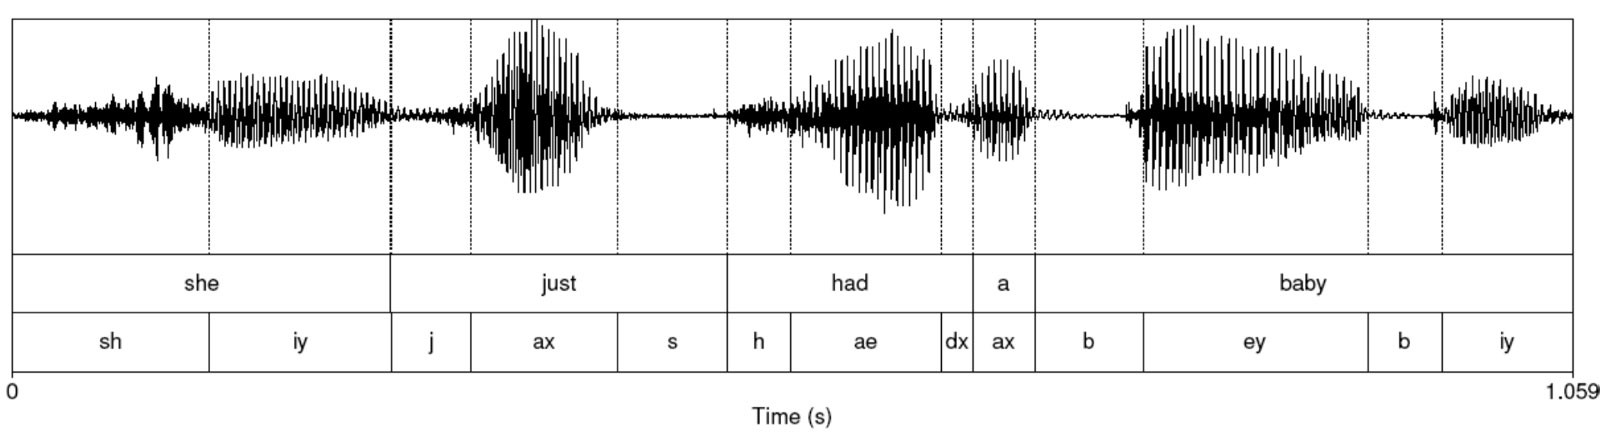
\includegraphics{phonems} 

}

\caption{Waveform of someone saying: 'she just had a baby '}\label{fig:phonemes}
\end{figure}

Audio is represented in a one-dimensional wave. Typical sample rates for
speech are: 8KHz, 16KHz, and each sample is typically 8-bit or 16-bit.
We can think of an audio signal as a one-dimensional vector
\(X = [x_1,x_2,....,x_n]\) representing time and a vector
\(Y = [y_1, y_2,...,y_n]\) representing the amplitude of the speech wave
\(y_i\) at time \(x_i\). However, this representation could change to a
different form (a spectrogram) that is covered in section
\ref{section:cnn}.

\hypertarget{how-asr-works}{%
\subsection{How ASR works}\label{how-asr-works}}

In a traditional ASR system, we would have an acoustic model whose job
is to learn the relationship between a sequence of phonemes and the
audio we are hearing. It accomplishes that by transforming speech
features to a conditional probability distribution over phones,
\(p(O|W)\). For instance, the pronunciation of the letter ``t'' at the
beginning of the word as ``tea'' and the end of it such as ``spirit,''
so, what is the probability of this letter being pronounced? There are
different elements involved in ASR systems apart from the acoustic
model, that are:

\noindent 

\textbf{Pronunciation dictionary} transforms phones into words. Every
word has a number of sounds representing it as in English dictionaries.
This could be affected by accent variation. In addition to that, the way
someone is speaking is also one of the factors affecting pronunciation
(spontaneous speech vs.~BBC radio news).\\
\textbf{Language model} represents a probability distribution over words
sequence, \(p(w)\). Language models solve the problem of listening
without being able to transform sounds to words or meanings, it assumes
audio is grammatically and semantically correct. It provides context to
distinguish between words and phrases that sound similar.\\
\textbf{Decoder} aggregates all knowledge to a contract search space, in
other words, the most probable word sequence. The job of the decoder is
to find the sequence of words \((W)\) that maximizes the probability of
a particular sequence \((w)\) given the audio \((X)\).

\begin{align}
\underset{W}{\operatorname{argmax}} P(W|X)
\end{align}

There have been many successful attempts to build acoustic models for
each language \protect\hyperlink{ref-phdthesis}{{[}13{]}}
\protect\hyperlink{ref-inproceedings}{{[}14{]}}
\protect\hyperlink{ref-inproceedings1}{{[}15{]}}. However, the
state-of-the-art is to build a language-independent acoustic model, but
also to increase the accuracy of existing models. Speaker independent
models are first trained from multiple speakers and then adapted to a
specific speaker either before or during recognition. Analogously,
language independent modeling is a methodology that combines speech and
models from multiple source languages and transforms them for
recognition in a specific target language
\protect\hyperlink{ref-859138}{{[}16{]}}. It is vital to mention that
speaking the same language with different accents might affect the
ability of that language's ASR system to recognize the speech.

\begin{figure}

{\centering 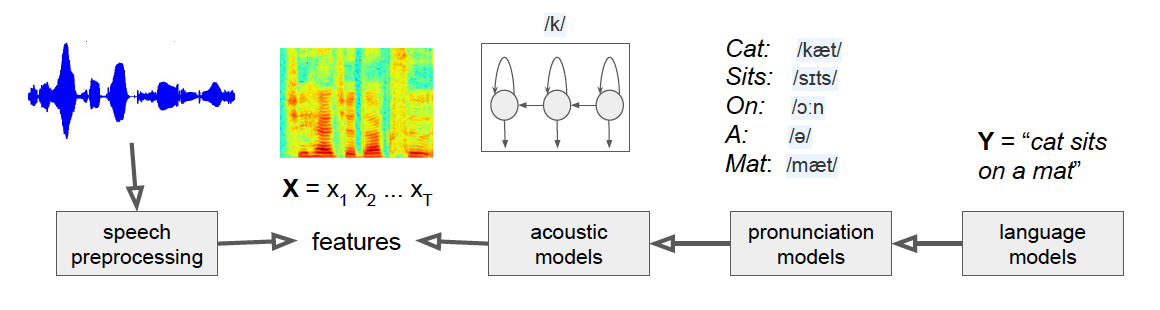
\includegraphics{classicway} 

}

\caption{The classic way of building a speech recognition system (https://heartbeat.fritz.ai/)}\label{fig:classicway}
\end{figure}

Figure \ref{fig:classicway} illustrates the classic way of building
speech recognition systems. A generative model of language is built, by
producing a certain sequence of words from the language model (rightmost
side), and then for each one of the words, the pronunciation model
decides how this particular word is spoken by writing in the form of
phonemes. The pronunciation models are then fed into an acoustic model
which decides how the phoneme sounds. The acoustic model does the
description through frames of audio features that are discussed next.

\hypertarget{speech-features-extraction}{%
\subsection{Speech Features
Extraction}\label{speech-features-extraction}}

Speech signals have high variability for many reasons including gender,
accent, emotion, and background noise. To reduce the variability of
speech signals some feature extraction should be done. There are many
feature extraction techniques used in speech recognition systems
including Linear predictive analysis (LPC), Linear predictive cepstral
coefficients (LPCC), Perceptual linear predictive coefficients (PLP),
Mel-frequency cepstral coefficients (MFCC), Power spectral analysis
(FFT), Mel scale cepstral analysis (MEL), Relative spectra filtering of
log domain coefficients (RASTA), and First-order derivative (DELTA)
\protect\hyperlink{ref-shrawankar2013techniques}{{[}17{]}}.

Mel-Frequency Cepstral coefficients (MFCC) is arguably the most used
feature for ASR including in deep learning (DL) systems. It is based on
short-time analysis (around 20--50 ms of sound), assuming speech to be
stationary during that period. MFCC shows good performances on clean
conditions, but it is not robust against speech distortions such as
background noise, reverberation, channel distortion, etc. One of the
reasons is because the log function is overly sensitive for low energy
spectra where much of speech information resides
\protect\hyperlink{ref-8949593}{{[}18{]}}.

\begin{align}
\label{eq:2}
C(x(t)) = F^{-1}[log(F[x(t)])]
\end{align}

Equation \ref{eq:2} shows how we can compute \emph{cepstrum} on top of
which MFCC is built, where \(x(t)\) is a signal in time domain (normal
waveform), \(F[x(t)]\) is the discrete fourier transform which generates
a spectrum by moving from time domain to frequency domain
\protect\hyperlink{ref-4320436}{{[}19{]}}. Fourier Transform transforms
a function of time \(x(t)\) to a function of frequency \(F[x(t)]\). Then
we apply logarithm on the amplitude of the spectrum for more
computational efficiency \protect\hyperlink{ref-logft}{{[}20{]}}.
Finally, we apply an inverse fourier transform to the log amplitude
spectrum to produce cepstrum.

\hypertarget{speech-classification}{%
\subsection{Speech Classification}\label{speech-classification}}

In ASR systems (illustrated in figure \ref{fig:classicway}), structured
sequence data is classified, where the label sequences are inferred from
the observation sequences. An accurate ASR system is a system that
performs with high accuracy in speech recognition tasks by classifying
label sequences (sentences) correctly from the observation sequences
(waveforms). We can model the posterior probability of the classes
directly in a discriminative model, whereas, in a generative model
Bayes' rule is used.

\hypertarget{generative-vs.-discriminative-classifier}{%
\subsubsection{Generative vs.~discriminative
classifier}\label{generative-vs.-discriminative-classifier}}

The model is to model the distribution of words in the word space. ASR
systems infer the sentences' acoustic waveforms. Speech signals are
sequential in nature, and that is where generative models come into view
by using Bayes' rule to combine Hidden Markov Model (HMM) acoustic
models and N-gram language models. On the contrary, the machine learning
and natural language processing (NLP) research areas are increasingly
dominated by discriminative approaches, where the class posteriors are
directly modeled \protect\hyperlink{ref-6296527}{{[}21{]}}. For
instance, when a child is told to ``bring that cup,'' the child does not
actually know unless one points to the cup, discriminative models would
tell the child the difference between the cup and the other objects that
might exist.

Generative model classification use Bayes' rule e.g., for HMMs, and it
can be split into a language model, the prior, \(P(w)\) that yields a
probability of any sentence, and an acoustic model
\(p(O_{1:T}| \lambda^{(w)})\) which is the likelihood that a sentence
\(w\) generated the observations \(O_{1:T}\) with model parameters
\(\lambda^{(w)}\). We can, as a result, obtain the posterior by applying
Bayes' rule:

\begin{align}
P(w|O_{1:T}, \lambda) = \frac{p(O_{1:T}|w, \lambda^{(w)}) P(w)}{\sum_{w}p(O_{1:T}|w, \lambda^{(w)})P(w)}
\end{align}

Whereas discriminative models directly model the posterior given the
observation sequence:

\begin{align}
P(w|O_{1:T}, \alpha) = \frac{1}{Z} \mathrm{exp} (\alpha^T \phi(O_{1:T}, w))
\end{align}

where \(Z\) is the normalization constant to ensure a valid probability
mass function over all sentences, and \(\alpha\) the discriminative
model parameters. \(\phi(O_{1:T}, w)\) is called the feature function.
Feature-function, shown in Figure \ref{fig:discriminative}, defines the
relationship between the sequence of observations and the sentence
label.

\begin{figure}

{\centering 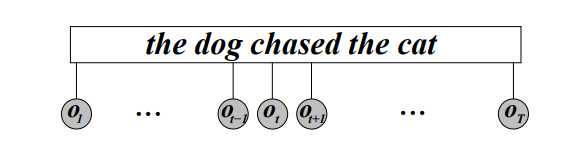
\includegraphics{discriminative} 

}

\caption{Graphical model for a simple discriminative model [13]}\label{fig:discriminative}
\end{figure}

\hypertarget{hmm-gmm-in-speech-recognition}{%
\subsection{HMM-GMM in Speech
Recognition}\label{hmm-gmm-in-speech-recognition}}

An acoustic model works as a human ear. Nearly four decades ago, the
expectation maximization (EM) algorithm was introduced as a principal
means for training HMMs which is a Markov Chain where the output symbols
or probabilistic functions that describe them, are connected either to
the states or to the transitions between states
\protect\hyperlink{ref-4815544}{{[}22{]}}. Both Hidden Markov Models
(HMM) and Gaussian Mixture Models (GMM) had been, before the era of deep
learning, must-learn technologies when dealing with speech signals.

HMMs are used as acoustic models to calculate the likelihood of
different classes generating observation sequences (sentences). HMM
model consists of hidden variables (States) and observables, a Markov
chain also contains the probability of transitioning from one state to
another. The modeling part, that is done by HMM, is for transitioning
between phonemes and the corresponding observable. GMM plays the role of
emission probability distribution which results in mixture emissions.
Figure \ref{fig:markov} shows Markov process and the transitioning
between different states.

\begin{figure}

{\centering 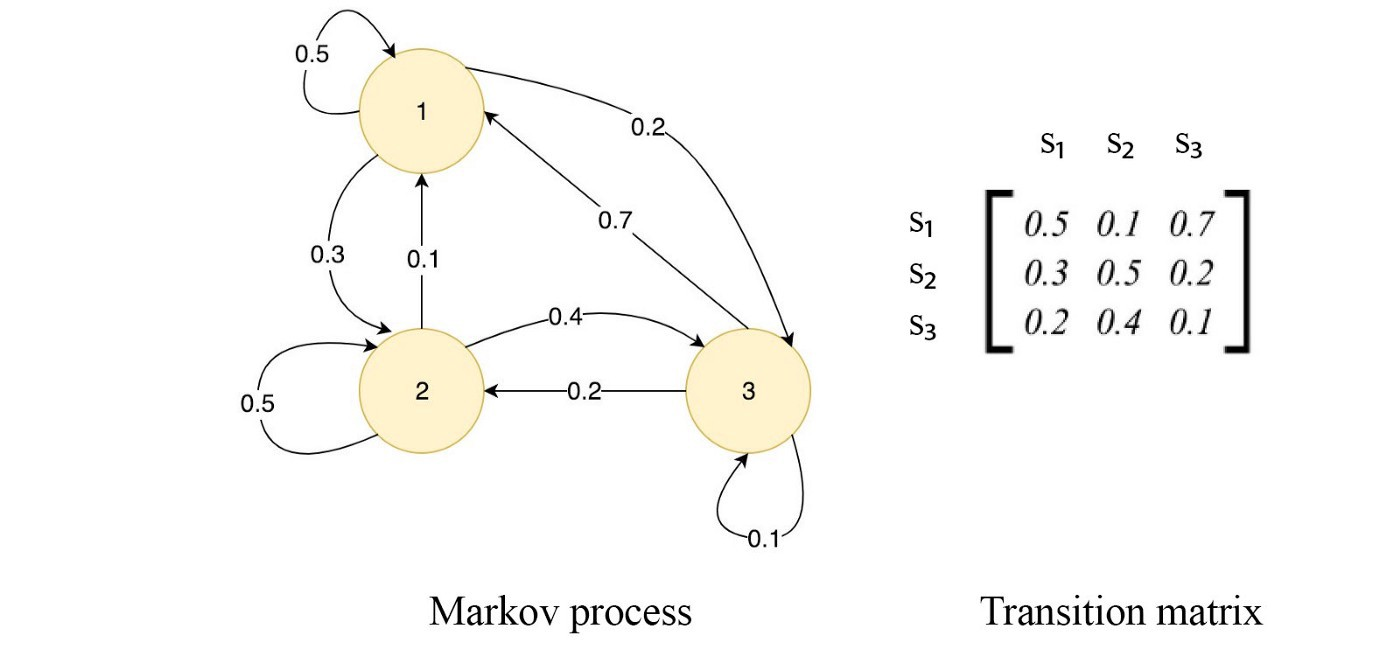
\includegraphics{markov} 

}

\caption{Markov Process and Transition Matrix}\label{fig:markov}
\end{figure}

Gaussian Mixture Models (GMMs) are, on the other hand, used to model the
distribution of features for phonemes. They allow modelling features
with a few possible values, which provides flexibility in speech
variations. In Figure \ref{fig:gmm}, it can be seen that when we try to
model the phone ``sh'' using gaussian model, it fixes the utterance of
that phoneme and does not allow for speech variations, whereas, when GMM
is used for the same purpose, it allows different pronunciations for the
same phone, which is more realistic for speech recognition.

\begin{figure}

{\centering 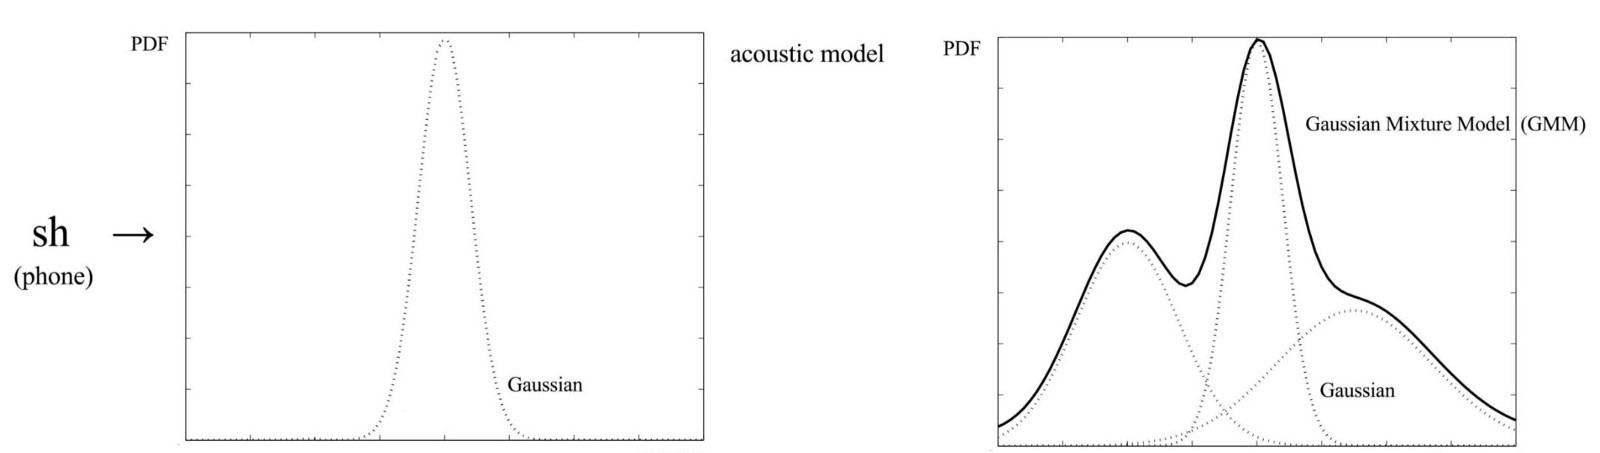
\includegraphics{gmm} 

}

\caption{Gaussian vs GMM acoustic model when modeling "sh"}\label{fig:gmm}
\end{figure}

\textbf{Pronunciation Model} For obtaining a good estimate for the
relationship between pronounced speech and the parts of words,
statistical models require an adequate number of samples. In order to
share information across words to avoid training statistical models on
each word (which is not feasible), the pronunciation model is used.

\begin{align}
\label{eq:3}
W^* = \underset{W}{\operatorname{argmax}} P(W|X)
\end{align}

By considering words as sequences of states \(Q\)

\begin{align}
W^* = \underset{W}{\operatorname{argmax}} P(X|Q, W) P(Q,W)
\end{align}

\begin{align}
W^* \approx \underset{W}{\operatorname{argmax}} P(X|Q) \sum_QP(Q|W) P(W)
\end{align}

\begin{align}
W^* \approx \underset{W}{\operatorname{argmax}} \underset{Q}{\operatorname{max}} P(X|Q) P(Q|W) P(W)
\end{align}

Where \(P(Q|W)\) is the pronunciation model
\protect\hyperlink{ref-pronun}{{[}23{]}}.

\textbf{Language Model} assigns a probability estimate to word
sequences, it is referred to in equation \ref{eq:4}, which is derived
from equation \ref{eq:3}, as \(P(W)\).

\begin{align}
\label{eq:4}
W^* = \underset{W}{\operatorname{argmax}} P(X|W) P(W)
\end{align}

The maximum likelihood estimate is calculated for estimating sequences
and is given by:

\begin{align}
P(w_i|w_1,...,w_{i-1}) = \frac{C(w_1, ..., w_i)}{\sum_v(C(w_1,...,w{i-1}v))}
\end{align}

Where \(C(w_1, ..., w_i)\) is the observed count in the training data.
For instance, if we want to know the probability of the word
(\emph{the}) being pronounced after the sentence (\emph{its water is so
transparent that}), this would give us:

\begin{align}
P(the|\text{its water is so transparent that}) = \frac{C(\text{its water is so transparent that the})}{\sum_vC(\text{its water is so transparent that})}
\end{align}

We can, hence, calculate the probability of the whole sequence by using
the chain rule as follows:

\begin{align}
P(w_1,...,wN) = \prod_{k=1}^N(w_k|w_{k-1})
\end{align}

\hypertarget{deep-learning-in-asr}{%
\subsection{Deep learning in ASR}\label{deep-learning-in-asr}}

DNNs have proven more successful in speech recognition than Gaussian
Mixture Model (GMM), and that is due to the fact that GMMs are
unsuitable for modeling data that resides on nonlinear manifolds or near
to them. For example, modeling the set of points that lie very close to
the surface of a sphere only requires a few parameters using an
appropriate model class, but it requires a very large number of diagonal
Gaussians or a fairly large number of full-covariance Gaussians
\protect\hyperlink{ref-6296526}{{[}24{]}}.

ASR systems rely on modern pipelines that are composed of many
processing stages, including specialized input features
\protect\hyperlink{ref-862023}{{[}25{]}}, acoustic models
\protect\hyperlink{ref-sak2015fast}{{[}26{]}}, and Hidden Markov Models
(HMMs) \protect\hyperlink{ref-5745027}{{[}27{]}}. Deep learning takes
the place of these processing stages and achieves higher performance
than traditional methods on hard speech
\protect\hyperlink{ref-hannun2014deep}{{[}3{]}}. An end-to-end deep
learning approach can replace entire pipelines of hand-engineered
components with neural networks, end to end learning allows us to handle
a diverse variety of speech including noisy environments, accents, and
different languages \protect\hyperlink{ref-amodei2015deep}{{[}28{]}}.
When deep neural networks are used, a considerable improvement is
acquired compared to that of GMM. An acoustic model can get between 10
and 20 percent relative improvement in accuracy
\protect\hyperlink{ref-inproceedings}{{[}14{]}}, which is a huge jump in
speech recognition and highly noticeable to a speaker. Achieving such
high accuracy in speech recognition tasks by using neural networks is,
in some sense, the first generation of deep learning in speech
recognition.

The hybrid deep neural network (DNN)- hidden Markov model (HMM) has been
shown to significantly improve speech recognition performance over the
conventional Gaussian mixture model (GMM)-HMM
\protect\hyperlink{ref-6857341}{{[}29{]}}. This could be attributed to
the fact that DNNs are capable of modeling complex correlations in
speech features.

\subsubsection{Convolutional Neural Networks for Speech Recognition}  
\label{section:cnn}

Convolutional Neural Networks (CNNs or ConvNet) are a class of deep
neural network that have many signal processing and computer vision
applications including speech recognition
\protect\hyperlink{ref-6857341}{{[}29{]}}. Rather than using fully
connected hidden layers that is similar to DNNs, CNNs present a network
structure consisting of \emph{convolutions} and \emph{pooling} layers.
The term convolution refers to combining two functions to yield a third
function, it is applied in CNNs to the input data by using a kernel or
filter to produce a feature map. A \emph{kernel} refers to the sets of
learnable parameters applied in convolution operation. Whereas, a
\emph{stride} is the distance between two successive kernel positions
\protect\hyperlink{ref-Yamashita2018}{{[}30{]}}. Figure \ref{fig:kernel}
shows how a simple \(3\times3\) kernel moves in a \(5\times5\) input
tensor with one stride \protect\hyperlink{ref-kernel}{{[}31{]}}, the
kernel moves across the input tensor one step to the right (the number
of strides) and it multiplies element-wise.

\begin{figure}

{\centering 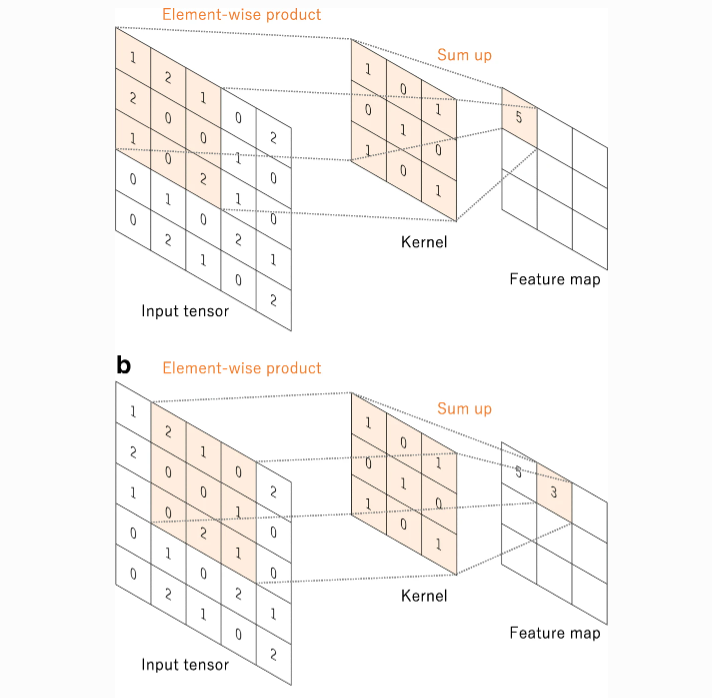
\includegraphics{kernel} 

}

\caption{A 3$\times$3 kernel with a 5$\times$5 input tensor and one stride}\label{fig:kernel}
\end{figure}

When using CNNs for speech recognition, speech signals can either be
transformed into spectrograms (images) or used as 1-d waves to organize
speech features into feature maps that are suitable for CNNs. Assuming
input feature maps are all one dimensional, each unit of one feature map
in the convolution ply can be computed as:

\begin{align}
\label{eq:7}
q_{j,m} = \sigma(\sum_{i=1}^I\sum_{n=1}^F o_{i,n+m-1}w_{i,j,n}+w_{0,j}), \ \ \ \ \ \ \ \ \ \ \ \ \ \ \ \ \ \ (j = 1,...,J)
\end{align}

Where \(o_{i,m}\) is the \emph{m}-th unit of the \emph{i}-th input
feature map, \(O_{i}\), \(q_{j,m}\) is the \emph{m}-th unit of the
\emph{j}-th feature map \(Q_j\) in the convolution ply, \(w_{i,j,n}\) is
the \emph{n}-th element of the weight vector, \(w_{i,j}\), that connects
the \emph{i}-th input feature map to the \emph{j}th feature map of the
convolution ply, \(F\) is the \emph{filter size}, which determines the
number of frequency bands in each input feature map that each unit in
the convolution ply receives as input.
\protect\hyperlink{ref-6857341}{{[}29{]}}. Equation \ref{eq:7} can
concisely be written in matrix form using the convolution operator \(*\)
as follows:

\begin{align}
\label{eq:9}
Q_j = \sigma(\sum_{i=1}^I O_i * \textbf{w}_{i,j}), \ \ \ \ \ \ \ \ \ \ \ \ \ \ \ \ \ \ (j = 1,...,J)
\end{align}

Where \(O_i\) is the \emph{i}-th input feature map and
\(\textbf{w}_{i,j}\) represents each local weight matrix. Figure
\ref{fig:fm} shows a pair of a convolution ply (on the left side) and a
pooling ply (rightmost), wherein, the mapping from either the input
layer or the pooling ply to a convolution ply is based on equation
\ref{eq:9} \protect\hyperlink{ref-6857341}{{[}29{]}}.

\begin{figure}

{\centering 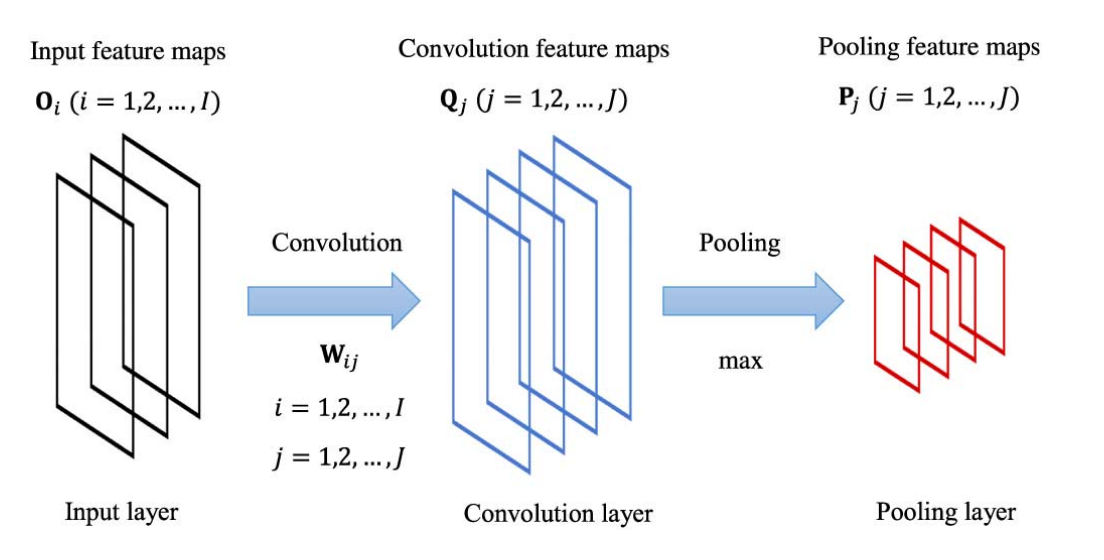
\includegraphics{fm} 

}

\caption{Two convolution plys and a pooling ply}\label{fig:fm}
\end{figure}

The limitation of this feature map is seen when a different feature map
is produced by a small stride (movement) in the feature position. This
limitation is addressed by \emph{downsampling}, and it is applied when
important structural elements are included in a lower resolution signal
which is generated from the input signal. To resolve this issue, a layer
of pooling is added after the convolutional layer. Pooling selects an
operation to be applied to the resulting feature maps, the result of
this operation is a reduction in the size of each feature map. When
using CNNs in image processing, the input is a (2-D) array of pixel
values at \emph{x} and \emph{y} axes, whereas, in speech signals, the
input could either be a spectrogram (Figure \ref{fig:spectrogram}) or it
could take a waveform. The temporal behavior of speech signals makes it
a fertile area for Temporal Convolutional Network (TCN) that uses the
convolutions for sequential speech data
\protect\hyperlink{ref-lemaire2019temporal}{{[}32{]}}.

\begin{figure}

{\centering 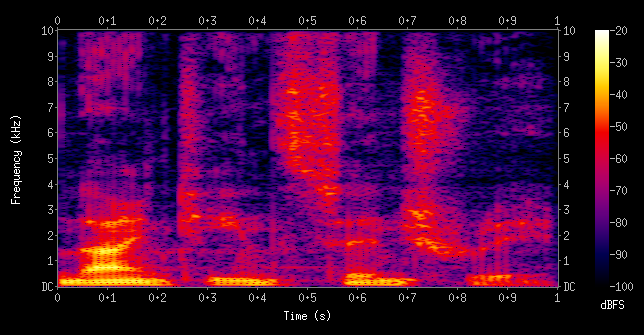
\includegraphics{spectrogram} 

}

\caption{A visual representation of the spectrum of frequencies of speech signal varying with time (Spectrogram) that is fed to CNNs}\label{fig:spectrogram}
\end{figure}

\hypertarget{recurrent-neural-networks-rnns-for-speech-recognition}{%
\subsubsection{Recurrent Neural Networks (RNNs) for Speech
Recognition}\label{recurrent-neural-networks-rnns-for-speech-recognition}}

An RNN is a class of Artificial Neural Networks (ANNs) that uses
sequential data or time series data. RNNs do not assume independence
between the current input and previous input, the output of RNNs depends
on the memorized prior sequence. For a given input sequence
\(x = (x_1, ..., x_T)\), a standard recurrent neural network computes
the hidden vector sequence \(h = (h_1, ..., h_T)\) and outputs vector
sequence \(y = (y_1, ..., y_T)\) by iterating the following equations
from \(t= 1\) to \(T\):

\begin{align}
h_t = \mathcal{H}(W_{xh} x_t + W_{hh} h_{t-1} + b_h)
\end{align}

\begin{align}
y_t = W_{hy} h_t + b_y
\end{align}

where the \(W\) terms denote weight matrices (e.g.~\(W_{xh}\) is the
input-hidden weight matrix), the b terms denote bias vectors
(e.g.~\(b_h\) is hidden bias vector) and \(\mathcal{H}\) is the hidden
layer function. \(\mathcal{H}\) is usually a sigmoid function,
nonetheless, the Long Short-Term Memory (LSTM)
\protect\hyperlink{ref-tian2017deep}{{[}33{]}}, which uses purpose-built
memory cells to store information, proved to be better at finding and
exploiting long range context than sigmoid function
\protect\hyperlink{ref-graves2013speech}{{[}34{]}}. It is implemented by
the following functions:

\begin{align}
\textit{$i_t = \sigma(W_{xi} X_t + W_{hi} h_{t-1} + W_{ci} c_{t-1} + b_i)$} \\
f_t = \sigma(W_{xf} X_t + W_{hf} h_{t-1} + W_{cf} c_{t-1} + b_f)\\
c_t = f_t c_{t-1} + i_t \tanh(W_{xc} x_t + W_{hc} h_{t-1} + b_c)\\
o_t = \sigma(W_{xo} X_t + W_{ho} h_{t-1} + W_{co} c_{t} + b_o)\\
h_t = o_t \tanh(c_t)
\end{align}

where \(\sigma\) is the logistic sigmoid function, and \(i\), \(f\),
\(o\) and \(c\) are input gate, forget gate, output gate and cell
activation vectors, respectively. Figure \ref{fig:rnn} illustrates the
Bidirectional RNNs (BRNNs) that computes the forward hidden sequence
\(\overrightarrow{h}\), the backward hidden sequence
\(\overleftarrow{h}\) and the output sequence \(y\) by iterating the
backward layer from \(t = T\) to 1, the forward layer from \(t = 1\) to
\(T\), and then updating the output layer. If BRNN is combined with
LSTM, it results in bidirectional LSTM which accesses both input
directions.

\begin{align}
\overrightarrow{h_t} = \mathcal{H}(W_{x\overrightarrow{h}} x_t + W_{\overrightarrow{h}\overrightarrow{h}} \overrightarrow{h_{t-1}} + b_{\overrightarrow{h}})\\
\overleftarrow{h_t} = \mathcal{H}(W_{x\overleftarrow{h}} x_t + W_{\overleftarrow{h}\overleftarrow{h}} \overleftarrow{h_{t+1}} + b_{\overleftarrow{h}})\\
h_t = W_{\overrightarrow{h}y} \overrightarrow{h_t} + W_{\overleftarrow{h} y} \overleftarrow{h_t} + b_y
\end{align}

\begin{figure}

{\centering 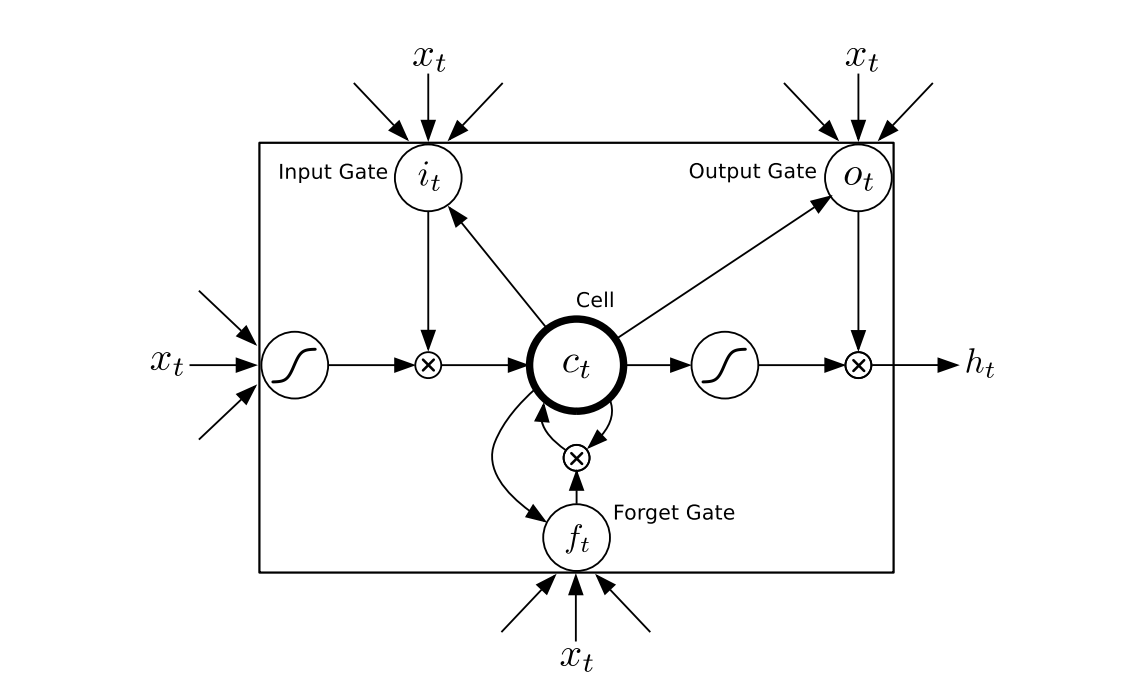
\includegraphics{lstm} 

}

\caption{Long Short-term Memory Cell}\label{fig:lstm}
\end{figure}

\begin{figure}

{\centering 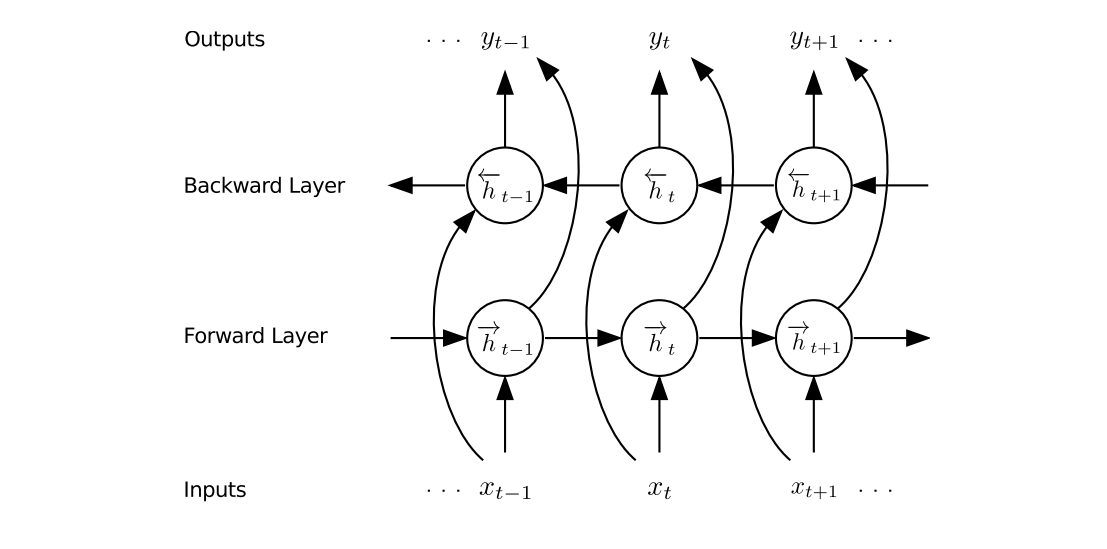
\includegraphics{rnn} 

}

\caption{Bidirectional RNN}\label{fig:rnn}
\end{figure}

\subsubsection{Transformers in Speech Recognition}  
\label{section:transformers}

The concept of transformers was proposed in 2017 for Natural Language
Processing (NLP) \protect\hyperlink{ref-vaswani2017attention}{{[}35{]}}.
It has, since then, been heavily used to solve different NLP tasks such
as text classification and text analysis. Transformers achieved 28.4
Bilingual Evaluation Understudy (BLEU) on the Workshop on Statistical
Machine Translation (WMT) dataset 2014, English-to-German translation
task, improving over the existing best results, including ensembles, by
over 2 BLEU \protect\hyperlink{ref-vaswani2017attention}{{[}35{]}}. In
machine translation systems, BLUE is a performance evaluation technique
that compares the candidate translation, which is done by the machine,
and the reference translation or the human-generated translation. For
speech recognition, Transformers have achieved competitive recognition
accuracy compared to RNN-based counterparts within both end-to-end and
hybrid frameworks \protect\hyperlink{ref-lu2020exploring}{{[}36{]}}.
Transformers are similar to RNNs in that they handle sequential input
data, but they, yet differ from RNNs in that they do not require
sequential data to be processed in order. They introduced an attention
mechanism that learns contextual relations between words (or sub-words)
in a text. The Transformer, in its most basic form, consists of an
encoder and a decoder, the encoder reads the text input by mapping an
input sequence of symbol representation \((x_1,...,x_n)\) to a sequence
of continuous representation \(z = (z_1,...,z_n)\) whereas, the decoder
produces a prediction for the task by generating an output sequence
\((y_1, ...,y_m)\) from the input \(z\) it receives from the encoder. As
opposed to directional models, which read the text input sequentially
(left-to-right or right-to-left), the Transformer encoder reads the
entire sequence of words at once. This bidirectional characteristic
allows the model to learn the context of a word based on all of its
surroundings (left and right of the word)
\protect\hyperlink{ref-towardsdatasience}{{[}37{]}}.

In speech recognition tasks, Transformers can achieve around 6\%
relative word error rate (WER) reduction compared to the bidirectional
LSTM (BLSTM) baseline in the offline fashion, where the entire speech
utterance is required as input for the encoder-decoder architecture. On
the other hand, in the streaming fashion, where the entire speech is not
available, Transformer-XL is comparable to latency-controlled BLSTM
(LCBLSTM) with 800-millisecond latency constraint
\protect\hyperlink{ref-lu2020exploring}{{[}36{]}}. Transformer-XL was
introduced in 2019 for the purpose of enabling learning dependency
without the fixed-length limitation and by keeping the temporal
coherence intact. It does that by using a segment-level recurrence
mechanism and a novel positional encoding scheme
\protect\hyperlink{ref-dai2019transformerxl}{{[}38{]}}.

\hypertarget{self-supervised-learning-ssl}{%
\subsection{Self-supervised Learning
(SSL)}\label{self-supervised-learning-ssl}}

Neural networks depend on enormous quantities of labeled data to learn,
and this scenario doesn't resemble the way humans learn. Self-supervised
learning has arisen as a machine learning worldview to solve the problem
of labeled data scarcity. It enables learning general data
representations from unlabeled examples in a supervised learning task
and fine-tunes the model on labeled data
\protect\hyperlink{ref-2020arXiv200611477B}{{[}2{]}} by adding a
predictor to the model that takes in the representations learned by SSL.
SSL provides, when pre-training on unlabeled data, effective contextual
audio representation. Additionally, by not relying on labels, SSL can
avoid many problems related to labels or audio files corruption, and
thus, increase model robustness. Moreover, self-supervision greatly
benefits out-of-distribution detection on difficult, near-distribution
outliers, to an extent that it exceeds the performance of fully
supervised methods
\protect\hyperlink{ref-2019arXiv190612340H}{{[}39{]}}. This has been
proven successful for natural language processing
\protect\hyperlink{ref-peters2018deep}{{[}40{]}}--\protect\hyperlink{ref-devlin2019bert}{{[}42{]}}
and is an active area of research in computer vision
\protect\hyperlink{ref-2020arXiv200611477B}{{[}2{]}}.

The elemental idea for SSL is to form some auxiliary pre-text task from
the input data and then feed it to the model such that while solving the
auxiliary task the model learns the underlying structure of the data
(object structure in an image). The model is trained to distinguish a
sample \(\mathrm{z}_{i+k}\) that is \(k\) steps ahead of distractor
samples \(\hat{\mathrm{z}}\) drawn from a distribution \(p_n\), it
performs this distinction by minimizing the contrastive loss (covered in
the next section) for steps \(k = 1,...,K\).

\subsubsection{Contrastive Learning}  
\label{section:cl}

In its simplest form, contrastive learning means for any positive pairs
(different views of the same data) of input \((x_1, x_2)\), there is a
pair of output functions \((f(x_1), f(x_2))\), a neural network function
in this context, that are similar to each other. And for a negative
input \(x_3\) both \(f(x_1)\) and \(f(x_2)\) are dissimilar to
\(f(x_3)\), Figure \ref{fig:cl}.

\begin{figure}

{\centering 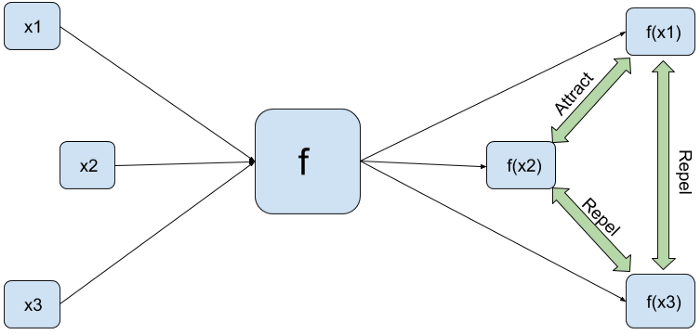
\includegraphics{cl} 

}

\caption{Contrastive Learning}\label{fig:cl}
\end{figure}

In a speech signal context, for an output \(c_t\), in order for the
model to know the true quantized latent speech representation \(q_t\) in
a set of \(K +1\) quantized candidate representations
\(\tilde{q} \in Q_t\) which includes \(q_t\) and \(K\) distractors.
These distractors are masked uniformly sampled time steps of the same
utterance. The loss is calculated as follows:

\begin{align}
\mathcal{L} = -log \frac{\exp(sim(c_t, q_t)/ k)}{\sum_{\tilde{q}\sim{Q_t}} \exp(sim(c_t, \tilde{q})/ k)}
\end{align}

\noindent where

\begin{align}
sim(c_t, q_t) = \frac{c_t . q_t}{||c_t|| \times ||q_t||} = \frac{\sum_{i=1}^n{c_{ti} . q_{ti}}}{\sqrt{\sum_{i=1}^n{c_{ti}^2}} \times \sqrt{\sum_{i=1}^n q_{ti}^2}}
\end{align}

\noindent \(sim(c_t, q_t)\) and \(sim(c_t, \tilde{q_t})\) are the cosine
similarity between context representations and quantized latent speech
representations
\protect\hyperlink{ref-he2020momentum}{{[}43{]}}\protect\hyperlink{ref-chen2020simple}{{[}44{]}}.
Low loss indicated high similarity between \(c_t\) and \(q_t\), whereas
high loss is a low similarity between them.

\hypertarget{ssl-in-speech-recognition}{%
\subsubsection{SSL in Speech
Recognition}\label{ssl-in-speech-recognition}}

A speech file consists of raw audio that could be represented as an
audio wave. In the framework used in this research (\emph{wav2vec 2.0})
\protect\hyperlink{ref-2020arXiv200611477B}{{[}2{]}}, a multi-layer
Convolutional feature encoder \(f: \mathcal{X}\to\mathcal{Z}\) is used
to encode raw speech audio \(\mathcal{X}\) and output latent speech
representations \(z_1,...,z_T\) for \emph{T} time-steps
\protect\hyperlink{ref-jiang2019improving}{{[}45{]}}. The output of the
feature encoder is discretized to \(\mathrm{q}_t\) and, thereafter, fed
to a Transformer network (discussed in section
\ref{section:transformers}) \(g: \mathcal{Z}\to\mathcal{C}\) to build
representations \(c_1,...,c_T\) by reading the entire sequence of words
at once (bidirectionally)
\protect\hyperlink{ref-devlin2019bert}{{[}42{]}}. The model is trained
via a contrastive task discussed in section \ref{section:cl}, defined
over a quantization of the latent representation, where the true latent
is to be distinguished from distractors
\protect\hyperlink{ref-2020arXiv200611477B}{{[}2{]}}.

\begin{figure}

{\centering 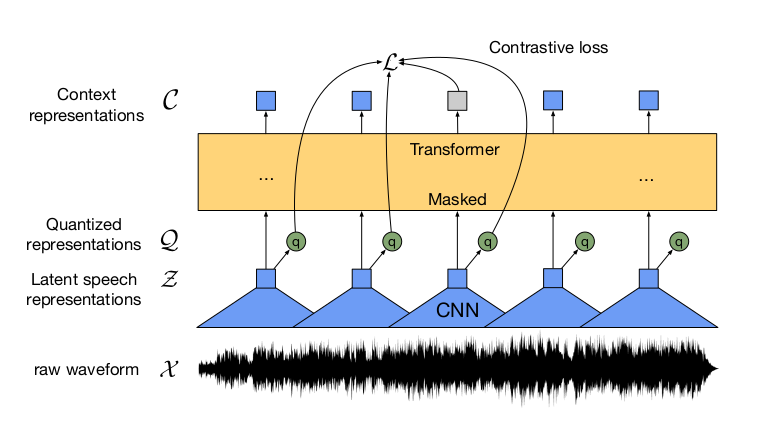
\includegraphics{framework2} 

}

\caption{The framework which jointly learns contextualized speech representations and an inventory of discretized speech units. [1]}\label{fig:framework}
\end{figure}

Figure \ref{fig:framework} illustrates how the model learns
contextualized speech representation. The model starts with raw audio (a
1-d waveform) that is used to feed a multi-layer feature encoder that
learns the representations (\(\mathcal{Z}\)). These representations are
vectors representing different wave segments, and are, then, transformed
into quantized representations \((\mathcal{Q})\) that are extracted from
multiple codebooks using product quantization
\protect\hyperlink{ref-5432202}{{[}46{]}}. These codebooks (illustrated
in figure \ref{fig:codebook}) are vectors in a \(d\)-dimensional space
containing vectors of codewords
\protect\hyperlink{ref-dieleman2018challenge}{{[}47{]}}. Given multiple
codebooks \(G\) with \(V\) entries \(e \in \mathbb{R}^{v\times{d}/G}\)
one entry is chosen from each codebook, the resulted vectors
\(e_1,...,e_G\) are concatenated and a linear transformation is applied
\(\mathbb{R}^d \to \mathbb{R}^f\) to obtain \(q \in \mathbb{R}^f\)
\protect\hyperlink{ref-2020arXiv200611477B}{{[}2{]}}. The extraction
mechanism depends on the shortest distance between the \(z\) vector and
\(q\) vectors. A Transformer is used to learn contextualized
representation by masking out some of the vectors \((\mathcal{Q})\) and
measuring the distance between the context \((\mathcal{C})\) and the
quantized \((\mathcal{Q})\) representations of those vectors by
calculating a contrastive loss.

\begin{figure}

{\centering 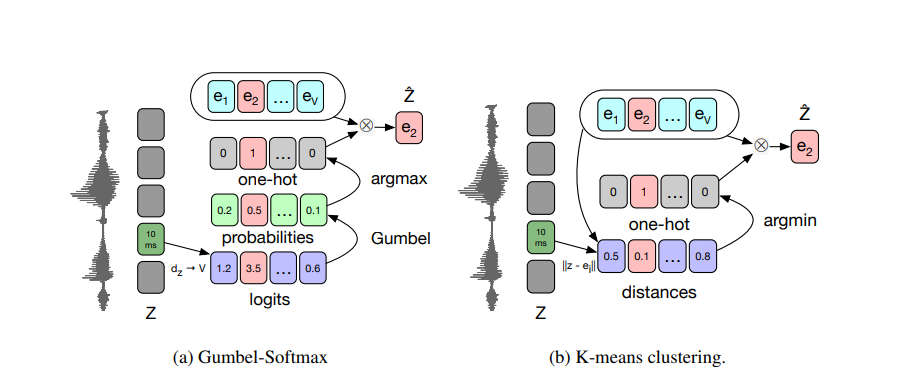
\includegraphics{codebook} 

}

\caption{Codebook generation using Gumbel-Softmax quantization}\label{fig:codebook}
\end{figure}

Figure \ref{fig:codebook} shows how Gumbel-Softmax which is a
differentiable approximation of the argmax is used for calculating
logits representing the codebook vectors. Gumbel-Softmax enables
selecting discrete codewords in a differentiable way. Given a latent
representation \(z\), a linear layer is applied, followed by a ReLU
\protect\hyperlink{ref-agarap2019deep}{{[}48{]}} and another linear
which outputs \(l \in \mathbb{R}^V\) logits for the Gumbel-Softmax. The
largest index in \(l\) is picked during inference. And the output
probabilities for choosing the \(j\)-th variable during training are:

\begin{align}
p_j = \frac{\mathrm{exp}(l_j + v_j)/\mathcal{T}}{\sum_{k=1}^V \mathrm{exp(l_k + v_k)/\mathcal{T}}}
\end{align}

Where \(v = -\mathrm{log}(-\mathrm{log}(u))\) and \(u\) are uniform
samples from \(\mathcal{U}(0,1)\)
\protect\hyperlink{ref-baevski2020vqwav2vec}{{[}10{]}}

\hypertarget{transfer-learning-tl}{%
\subsubsection{Transfer Learning (TL)}\label{transfer-learning-tl}}

Transfer learning is to use a model, that was used for a specific task,
for a new related task as a starting point. It stores the knowledge it
gained while solving the initial task, and then uses that knowledge for
a different but related task. In speech recognition, we can refer to the
initial task as ``source language'' and the new task as ``target
language,'' thus, we can initialize the network for the target language
with a pre-trained model from the source language. TL has been shown to
be able to improve the performance and considerably decrease WER
\protect\hyperlink{ref-joshi2020transfer}{{[}49{]}}.

\hypertarget{pre-trained-models}{%
\subsubsection{Pre-trained Models}\label{pre-trained-models}}

\hypertarget{wav2vec-pre-training}{%
\paragraph{\texorpdfstring{WAV2VEC Pre-training
\newline \newline}{WAV2VEC Pre-training }}\label{wav2vec-pre-training}}

\emph{wav2vec} is a model for unsupervised pre-training tasks in speech
recognition developed by Facebook AI. It is a multi-layer convolutional
neural network (CNN) that receives raw audio as input and outputs
general representations for the raw audio, which can subsequently be
used as input to ASR systems. WAV2VEC reduces WER of a strong
character-based log-mel filterbank baseline
\protect\hyperlink{ref-m2014choice}{{[}50{]}} by up to 36 \% when only a
few hours of transcribed data is available
\protect\hyperlink{ref-schneider2019wav2vec}{{[}51{]}}. Figure
\ref{fig:wav2vec} shows the architecture of WAV2Vec that takes the raw
audio as input to a fully connected CNN to solve the next time
prediction task.

\begin{figure}

{\centering 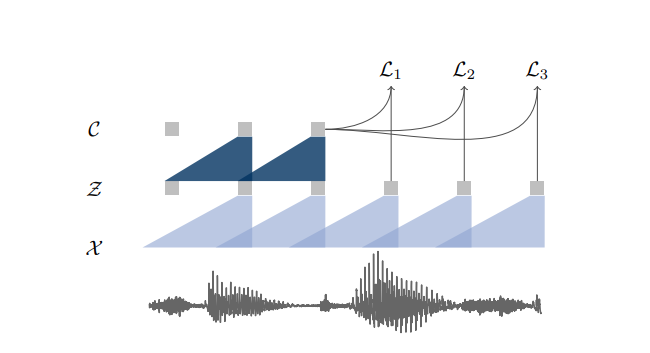
\includegraphics{wav2vec} 

}

\caption{WAV2VEC Fully Convolutional Architecture [35]}\label{fig:wav2vec}
\end{figure}

The parameterized encoder network
\(f : \mathcal{X} \mapsto \mathcal{Z}\) is applied on the raw audio
samples \(x_i \in \mathcal{X}\). With kernel sizes of (10, 8, 4, 4, 4)
and strides of (5, 4, 2, 2, 2), The output of the encoder is a
low-frequency feature representation \(\mathrm{z}_i \in \mathcal{Z}\)
which encodes about 30 milliseconds of 16 kHz of audio and the striding
results in representations \(\mathrm{z}_i\) every 10ms
\protect\hyperlink{ref-schneider2019wav2vec}{{[}51{]}}.

The output of the encoder network is then fed into a context network
\(g : \mathcal{Z} \mapsto \mathcal{C}\) which can be seen in figure
\ref{fig:framework}, and that has nine layers with kernel size three,
stride one, and 210 ms receptive field. The context network outputs a
single contextualized tensor
\(c_i = g(\mathrm{z_i}... \mathrm{z_{i-v}})\) from the multiple latent
representations \(\mathrm{z_i}... \mathrm{z_{i-v}}\) obtained from the
encoder network. This context network follows the Transformer
architecture \protect\hyperlink{ref-2020arXiv200611477B}{{[}2{]}}. An
output layer is added on top of the transformer network to fine-tune the
model on labeled data and make predictions.

\hypertarget{cross-lingual-speech-representation-xlsr}{%
\paragraph{\texorpdfstring{Cross-lingual Speech Representation (XLSR)
\newline \newline}{Cross-lingual Speech Representation (XLSR) }}\label{cross-lingual-speech-representation-xlsr}}

As opposed to pre-training speech models on one language (monolingual
pre-training), it is also feasible to make use of data from other
languages for performance improvement. This has worked well for natural
language processing, by achieving state-of-the-art results on
cross-lingual classification, unsupervised and supervised machine
translation \protect\hyperlink{ref-lample2019crosslingual}{{[}52{]}}.
Learning cross-lingual speech representation in pre-training is not only
possible, but it also outperforms monolingual models in many
experiments. XLSR showed a relative phoneme error rate reduction of 72\%
compared to the best known results, and it also improved word error rate
by 16\% On BABEL corpus compared to a comparable system
\protect\hyperlink{ref-conneau2020unsupervised}{{[}53{]}}. This
pre-trained XLSR model is finetuned on individual languages which
results in a different model for each language. This is particularly
useful for languages with low resources as it uses other languages'
resources plus the low amount of data from the target language for
pre-training, then fine-tune it on the target language.

\begin{figure}

{\centering 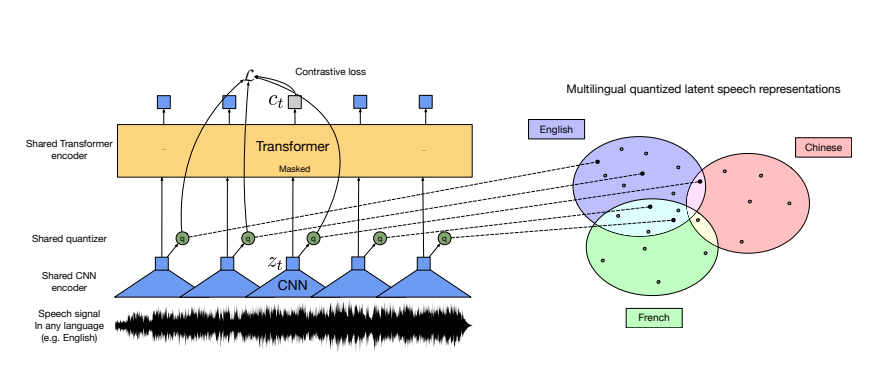
\includegraphics{xlsr} 

}

\caption{Cross-lingual Speech Representation (XLSR) Approach [36]}\label{fig:xlsr}
\end{figure}

Figure \ref{fig:xlsr} shows the approach of XLSR which is similar to
that of WAV2VEC, and that is because of the fact that XLSR is built on
top of WAV2VEC framework. Nevertheless, in XLSR architecture, it could
be seen that the speech signals of different languages are fed to the
shared encoder, which then produces the latent representations
\(\mathcal{Z_t}\). The latent representations for all languages are then
quantized using a shared quantizer, these quantized representations
\(q_1 ...q_n\) are then fed to a shared transformer network (encoder) by
masking some of the quantized vectors out. The contrastive loss is
calculated after that in the same way it is calculated in WAV2VEC,
except, in XLSR it is calculated for the output of the shared encoder.
The representations produced by the transformer network that are learnt
with SSL are then used as input to an additional function that can be
trained with regular supervised learning in the fine-tuning phase.

\hypertarget{connectionist-temporal-classification-ctc}{%
\subsection{Connectionist Temporal Classification
(CTC)}\label{connectionist-temporal-classification-ctc}}

CTC is an algorithm used to solve the issue of the mismatch between the
true written sentence and the predicted sentence, it uses the history of
the target character without assuming conditional independence between
characters. In the bottom of Figure \ref{fig:ctc} we can see how CTC
classifies a speech signal, the shaded lines are the output activations,
and they correspond to the probability of phonemes matches at particular
times. The CTC network predicts only the sequence of phonemes (typically
as a series of spikes, separated by `blanks,' or null predictions),
while the framewise network attempts to align them with the manual
segmentation (vertical lines)
\protect\hyperlink{ref-inproceedingsctc}{{[}54{]}}.

\begin{figure}

{\centering 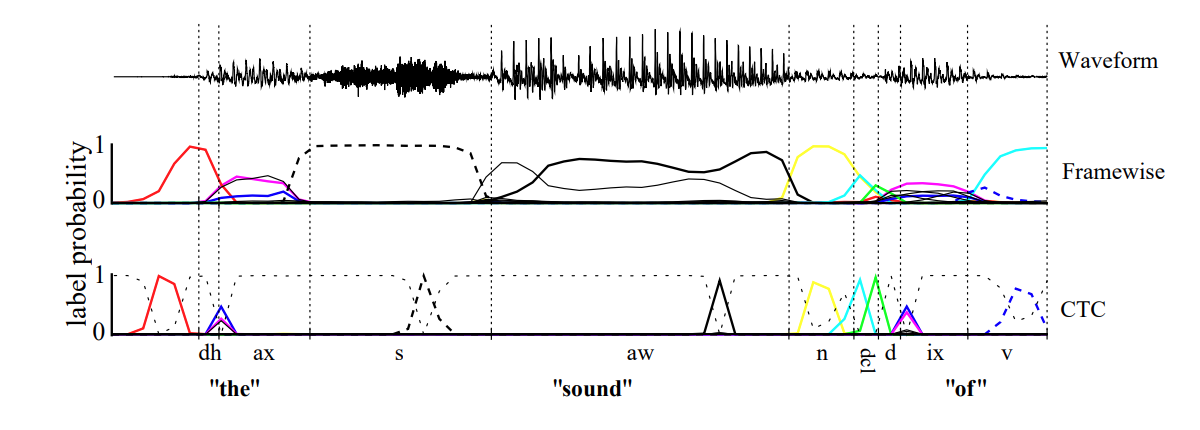
\includegraphics{ctc} 

}

\caption{Connectionist Temporal Classification (CTC)}\label{fig:ctc}
\end{figure}

\begin{align}
p(Y|X) = \sum_{A \in \mathcal{A}_{X,Y}} \prod_{t=1}^T p_t(a_t|X)
\end{align}

For a given input sequence \(X = [x_1, ..., x_T]\) and a corresponding
output sequence \(Y = [y_1, ..., y_U]\), CTC assigns probabilities for
each Y given an X. More specifically, it marginalizes over the set of
valid alignments and computes the probability for a single alignment
step-by-step. CTC does not require alignment between input and output
sequences, nonetheless, it sums over the probability of all possible
alignments to get the probability of an output given an input.

\emph{Loss Function } CTC loss function is used when fine-tuning the
model for evaluating the quality of the self-supervised pre-training
phase, the aim is to maximize the probability of the correct alignment
between input \(x_i\) and output \(y_i\) or to compute the conditional
probability \(p(Y|X)\). Then to infer a likely \(Y\) given \(X\) as
follows:

\begin{align}
Y^* = \underset{Y}{\operatorname{argmax}} P(Y|X)
\end{align} CTC assigns probabilities for each \(Y\) given an \(X\)
according to the alignments between inputs and outputs. Since alignment
between input and output is not required by CTC, this makes it suitable
for speech input which can have stretches or silence that do not
correspond to output. CTC introduces a blank token \(\epsilon\) to the
set of allowed output, this \(\epsilon\) is a placeholder and removed
from the output. Figure \ref{fig:epsilon} shows how \(\epsilon\) is
introduced in the word hello, where repeating characters are merged
first, then any \(\epsilon\) is removed and the remaining characters are
the output. In figure \ref{fig:prob} it can be seen that for an input of
audio signal, the input could be fed into RNN or a CNN where the network
gives \(p_t(a|X)\) a distribution over the outputs \{h, e, l, o,
\(\epsilon\)\} for each input step, the probability of different
sequences is then calculated \protect\hyperlink{ref-ctc}{{[}55{]}}. The
alignment of the most likely output can be calculated by getting the
highest probable alignment as follows:

\begin{align}
\underset{A}{\operatorname{argmax}} \prod_{t=1}^Tp_t(a_t|X)
\end{align}

\begin{figure}

{\centering 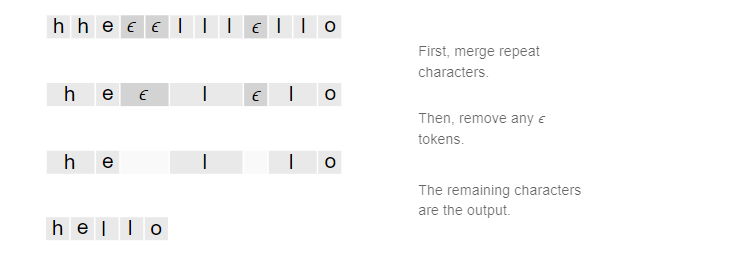
\includegraphics{epsilon} 

}

\caption{$\epsilon$ Introduction into the word hello}\label{fig:epsilon}
\end{figure}

\begin{figure}

{\centering 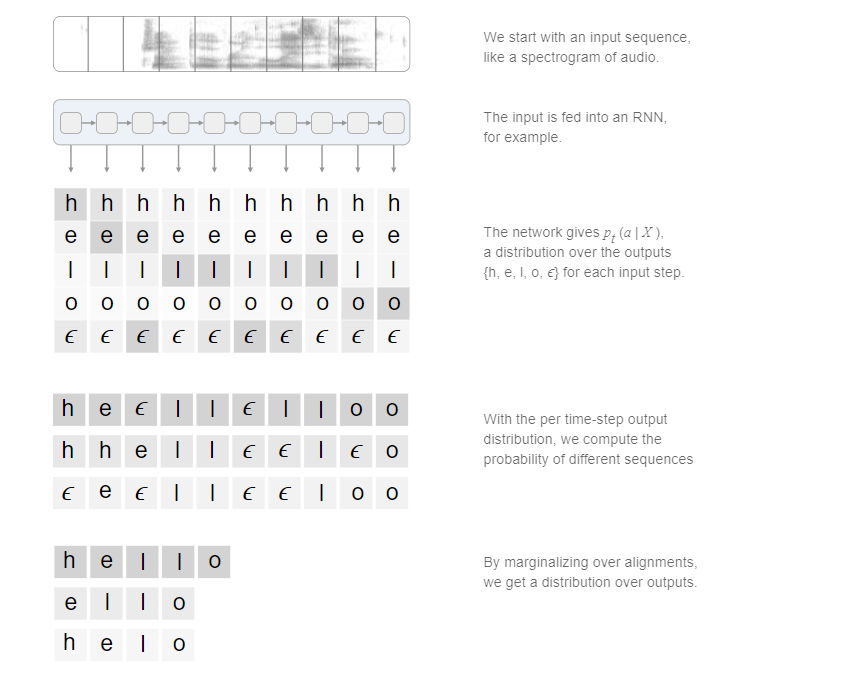
\includegraphics{prob} 

}

\caption{How CTC assigns probabilities}\label{fig:prob}
\end{figure}

\hypertarget{asr-models-evaluation}{%
\subsection{ASR Models Evaluation}\label{asr-models-evaluation}}

The error rate of the predicted transcript is calculated as a
measurement of how accurate an ASR is. The purpose of this process is to
compare the performance of different models and techniques, but it can
also go as deep as calculating the performance of these models with
different hyperparameters settings. When evaluating an ASR we compare
the output of the ASR system with the literal transcription of the input
audio. The performance of ASRs depends on several factors including
audio recording condition (e.g.~background noise or the recording
channel noise), spoken language variability (e.g.~spontaneous speech,
formal speech, or different accents or dialects), or the speaker
variability (e.g.~men and women, a speaker in different conditions such
as illness, different emotions, and tiredness).

There are two key areas related to ASR errors, the first one is the
reference-recognised alignment which consists of finding the best word
alignment between the reference and the automatic transcription and the
second one is the evaluation metrics measuring the performance of the
ASR systems \protect\hyperlink{ref-ERRATTAHI201832}{{[}56{]}}.

\hypertarget{reference-recognised-word-sequences-alignment-rrwsa}{%
\subsubsection{Reference-Recognised Word Sequences Alignment
(RRWSA)}\label{reference-recognised-word-sequences-alignment-rrwsa}}

RRWSA refers to comparing the referenced and recognised words for the
purpose of finding three types of errors. First, substitution error:
where a word in the reference word sequence is predicted as a different
word. Second, Deletion error: where a word could entirely be deleted in
the predicted transcript. The third error type is the Insertion error,
and in this error, a new word appears in the predicted transcript. This
word sequence alignment is normally calculated using Viterbi Edit
Distance \protect\hyperlink{ref-682181}{{[}57{]}}, in which the weighted
error score for the word sequence is minimized. Two distances are
calculated (shown in \ref{eq:dist1} and \ref{eq:dist2}), the first
distance (\(d_\phi^v(x^T,y^V)\)) is the most likely transduction between
the two strings that is calculated by taking the logarithm of the
probability of the most likely edit sequence for the string pair
\(\langle x^T,y^V\rangle\) and it is calculated recursively
\protect\hyperlink{ref-682181}{{[}57{]}}, whereas \(d_\phi^s(x^T,y^V)\)
is called the stochastic edit distance, and it aggregates all
transductions between the two strings by calculating the logarithm of
the probability of the string pair \(\langle x^T,y^V\rangle\) according
to the transducer \(\phi\).

\begin{align}
\label{eq:dist1}
d_\phi^{v}(x^T, y^V) = -\log \mathrm{max}_{\{ z^n : v(z^n) = \langle x^T, y^V \rangle \}} \{p(z^n|\phi) \}
\end{align}

\begin{align}
\label{eq:dist2}
d_\phi^{s}(x^T, y^V) = -\log  \ p(x^T, y^V|\phi)
\end{align}

The \textbf{Viterbi edit distance} calculates the probability of the
most likely edit sequence for a string pair (\(x^T, y^V\))

\hypertarget{word-error-rate-wer-evaluation-metric}{%
\subsubsection{Word Error Rate (WER) Evaluation
Metric}\label{word-error-rate-wer-evaluation-metric}}

Word Error Rate (WER) is the most popular metric for ASR evaluation, it
measures the percentage of incorrect words (Substitutions (S),
Insertions (I), Deletions (D)) regarding the total number of words
processed \protect\hyperlink{ref-ERRATTAHI201832}{{[}56{]}}.

\begin{align}
WER = \frac{S + D + I}{N} = \frac{S + D + I}{H + S + D}
\end{align}

where \emph{S} is the total number of words that were substituted, in
the predicted transcript, with other words, \emph{D} is the total number
of words that were deleted in the predicted transcript but they are in
the input transcript, \emph{I} is the total number of newly inserted
words into the predicted written words, \emph{N} is the total number of
input words, and \emph{H} is the total number of correct words.

\newpage

\hypertarget{data}{%
\section{Data}\label{data}}

The training data for the Language Model (LM) is limited, and many
require Natural Language Processing (NLP) tools such as morph analyzer,
diacritizer, and text normalizers to be developed
\protect\hyperlink{ref-Abdou_Moussa_2018}{{[}58{]}}. The data in this
thesis is downloaded from Mozilla Common Voice Corpus (6.1), the size of
the dataset is 2 GB with 49 validated hours by the community (the
community validates by either matching the voice with the written text
or speaking the text itself), 77 hours in total, 672 number of voices,
and mp3 audio format.

\hypertarget{how-mozilla-common-voice-community-validates}{%
\subsection{How Mozilla Common Voice Community
validates}\label{how-mozilla-common-voice-community-validates}}

Mozilla depends on contributors who record their voice clips by reading
a piece of text and record their voice, this voice is then queued for
validation. The clip is valid if another user listens to it and marks it
as valid, however, to have the clip in Common Voice dataset, it must be
validated by at least two users. If a clip gets a negative vote, it will
be returned to the queue, and if it gets another negative vote, then it
will be moved to the clip graveyard where all invalid clips exist.
\protect\hyperlink{ref-Mozilla}{{[}4{]}}

\hypertarget{data-preprocessing}{%
\subsection{Data Preprocessing}\label{data-preprocessing}}

\hypertarget{preprocessing-audio-files}{%
\subsubsection{Preprocessing Audio
Files}\label{preprocessing-audio-files}}

Since the dataset was initially mp3 audio files, all the files were
converted to wav files, the framework considers the following
conditions:

\begin{itemize}
\tightlist
\item
  The sample rate is to be changed to 16000
\item
  The Pulse-code modulation (PMC) is to also be changed to 16 bit
\item
  The silence should be removed from all audio files
\item
  Each audio file should contain only one person speaking
\end{itemize}

\hypertarget{preprocessing-transcripts}{%
\subsubsection{Preprocessing
Transcripts}\label{preprocessing-transcripts}}

The framework requires the transcript to be in the following format:

\begin{enumerate}
\def\labelenumi{\arabic{enumi}.}
\tightlist
\item
  One sample per line

  \begin{itemize}
  \tightlist
  \item
    The Arabic language is written from right to left (rtl language),
    hence, the sentences were reversed to meet the criteria for the
    transcript file.
  \end{itemize}
\item
  Upper case

  \begin{itemize}
  \tightlist
  \item
    The Arabic language does not have upper and lower case as English,
    therefore, this condition is ignored.
  \end{itemize}
\item
  All numbers should be transformed into verbal form.

  \begin{itemize}
  \tightlist
  \item
    All numbers found in the dataset were transformed to verbal form.
  \end{itemize}
\item
  All special characters (eg. punctuation) should be removed. The final
  text should contain words only.

  \begin{itemize}
  \tightlist
  \item
    All punctuation marks have been removed from the sentences according
    to what is required by the framework.
  \end{itemize}
\item
  Words in a sentence must be separated by whitespace character

  \begin{itemize}
  \tightlist
  \item
    All words in sentences were separated by whitespaces.
  \end{itemize}
\end{enumerate}

\hypertarget{diacretics}{%
\subsubsection{Diacretics}\label{diacretics}}

Diacritical marks play a crucial role in meeting the criteria of
usability of typographic text, such as homogeneity, clarity, and
legibility \protect\hyperlink{ref-hssini2011design}{{[}59{]}}.
Diacritics are placed above, below, or through a letter, and they can
change the semantic of a word completely, see Figure
\ref{fig:diacritics}.

\begin{figure}

{\centering 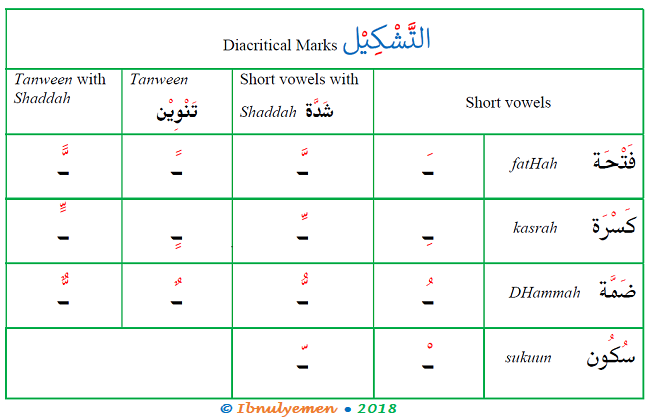
\includegraphics{diacritics} 

}

\caption{Diacritical marks in Arabic (https://blogs.transparent.com/arabic/basic-arabic-diacritical-marks/)}\label{fig:diacritics}
\end{figure}

All diacritics were removed from the sentences as they posed a problem
when training the model with them, the model read diacritics as
individual letters which affected the accuracy since it was required to
remove all punctuation marks from the sentences because the model learns
the meaning from the context and does not depend on individual words.

\newpage

\hypertarget{methodology}{%
\section{Methodology}\label{methodology}}

Self-supervised learning is used in this research with its two phases of
pre-training and fine-tuning, where transfer learning is the main
technique. The implementation is done on a cloud-hosted server with
Tesla K80 Nvidia GPU, using a wrapper version of wav2vec 2.0 framework
\protect\hyperlink{ref-2020arXiv200611477B}{{[}2{]}} that is used for
the purpose of training and testing the model. After the
\protect\hyperlink{data-preprocessing}{data preprocessing phase} of
Mozilla Common Voice Arabic dataset (6.1), two approaches were carried
out. The first one was to pre-train a monolingual model on the training
dataset and fine-tune it on the validation dataset, this model is then
tested on the test dataset. The second approach was to use a pre-trained
XLSR model and fine-tune it on training and validation datasets, then
the fine-tuned model is evaluated on the test dataset. The first
approach was inefficient because of the time and resources it took for
completing the pre-training phase, the model used in this approach had a
long pre-training time, it continued for more than 21 days and the
pre-training was ongoing until it was stopped with 58\% accuracy. It was
then decided to choose a pre-trained model that could be fine-tuned on
Arabic language (the second approach), the chosen model for this purpose
is a pre-trained Wav2Vec2-XLSR-53 that is pre-trained on 53 languages
including Arabic.

\hypertarget{data-preparation}{%
\subsection{Data Preparation}\label{data-preparation}}

The wrapper used for model training was used for the English language,
and it requires the transcript file to include the path to the wav files
and the transcript corresponding to the was file in one line. Since
English is a left-to-right (ltr) language and Arabic is a right-to-left
(rtl) language, the Arabic sentences are reversed to fit in the wrapper
requirements. Figure \ref{fig:english} illustrates the representation of
English in the English transcript file, whereas Figure \ref{fig:arabic}
demonstrates the reversed Arabic sentence in the Arabic transcript file.

\begin{figure}

{\centering 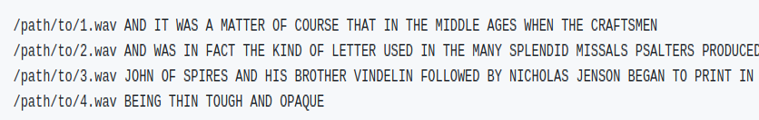
\includegraphics{english} 

}

\caption{a snippet of the English transcript file}\label{fig:english}
\end{figure}

\begin{figure}

{\centering 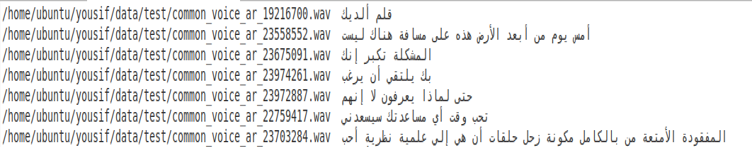
\includegraphics{arabic} 

}

\caption{a snippet of the Arabic transcript file}\label{fig:arabic}
\end{figure}

\hypertarget{pre-training-phase}{%
\subsection{Pre-training Phase}\label{pre-training-phase}}

During pre-training, representations of speech audio are learnt by
solving a contrastive task (see section \ref{section:cl}). The
pre-training phase requires having a set of distractors from which to
identify the correct quantized latent audio representation. This phase
took more than 21 days (504 hours), it was then stopped, after 662
epochs for the purpose of fine-tuning.

\begin{align}
\label{eq:1}
\frac{p(\mathrm{z_{i+k}}|\mathrm{z_i}...\mathrm{z_{i-r}})}{p(\mathrm{z_{i+k}})}
\end{align}

During the pre-training phase, the model predicts future samples from a
given signal context, this poses a challenge when modeling the data
distribution \(p(x)\) due to the difficulty associated with calculating
feature samples for high-frequency speech signals. To avoid this
problem, raw speech samples \(\mathrm{x}\) are encoded into a feature
representation \(\mathrm{z}\) at a lower temporal frequency, and then
equation \ref{eq:1} shows the density modeling ratio.

\hypertarget{fine-tuning-phase}{%
\subsection{Fine-tuning Phase}\label{fine-tuning-phase}}

After the pre-training phase, the model is fine-tuned on the labeled
dataset by adding an output layer on top of the Transformer network for
prediction. The model is optimized with Adam optimizer
\protect\hyperlink{ref-kingma2017adam}{{[}60{]}} with a batch size of
3.2 minutes samples.

\hypertarget{pre-trained-cross-language-model}{%
\subsection{Pre-trained Cross-language
Model}\label{pre-trained-cross-language-model}}

A second methodology is used in this research, where multilingual
pre-trained models are explored. The pre-trained model used is
XLSR-Wav2Vec2, the successor to wav2vec, this model learns basic speech
units used to tackle a self-supervised task for several languages, and
is pre-trained and released by Facebook AI Research in September 2020.
The pre-trained model is trained the same way \emph{wav2vec2.0} is, but
on 53 different languages. This model can benefit from the availability
of some languages and use them for less available languages.
XLSR-Wav2Vec2 is fine-tuned using CTC for calculating the loss by
summing up all scores of all possible alignments between input and
output.

XLSR-Wav2Vec2 model has many hyperparameters to tune, nonetheless, a
small number of these parameters, that we fine-tune during the
fine-tuning phase, is mentioned here:

\noindent  \textbf{save\_steps} is the number of update steps before two
checkpoint saves.\\
\textbf{eval\_steps} is when evaluation is done (and logged) by
calculating the WER.\\
\textbf{num\_train\_epochs} is the number of full iteration on our data
the neural network is going to perform.\\
\textbf{per\_device\_train\_batch\_size} is the batch size per GPU
core.\\
\textbf{gradient\_accumulation\_steps} is the number of updates steps to
accumulate the gradients for, before performing a backward/update
pass.\\
\textbf{save\_total\_limit} is the number of checkpoints to save.

\newpage

\hypertarget{result}{%
\section{Result}\label{result}}

\hypertarget{the-result-of-the-monolingual-model}{%
\subsection{The result of the monolingual
model}\label{the-result-of-the-monolingual-model}}

Figure \ref{fig:training_accuracy} shows training and validation
accuracies (which indicates how accurate the model predicts the true
masked vector) during pre-training on Mozilla Common Voice training
dataset. As it can be seen in the chart, the training accuracy was in a
very slow increase trend, whereas the validation accuracy never went
above 0.601 except for the first 50 warmup epochs. The validation
accuracy started to slightly decrease after around 450 epochs (in the
fifteenth day of pre-training). This accuracy refers to how good our
contrastive learning is, in other words, how accurate is our prediction
of the true masked vectors.

\begin{figure}

{\centering 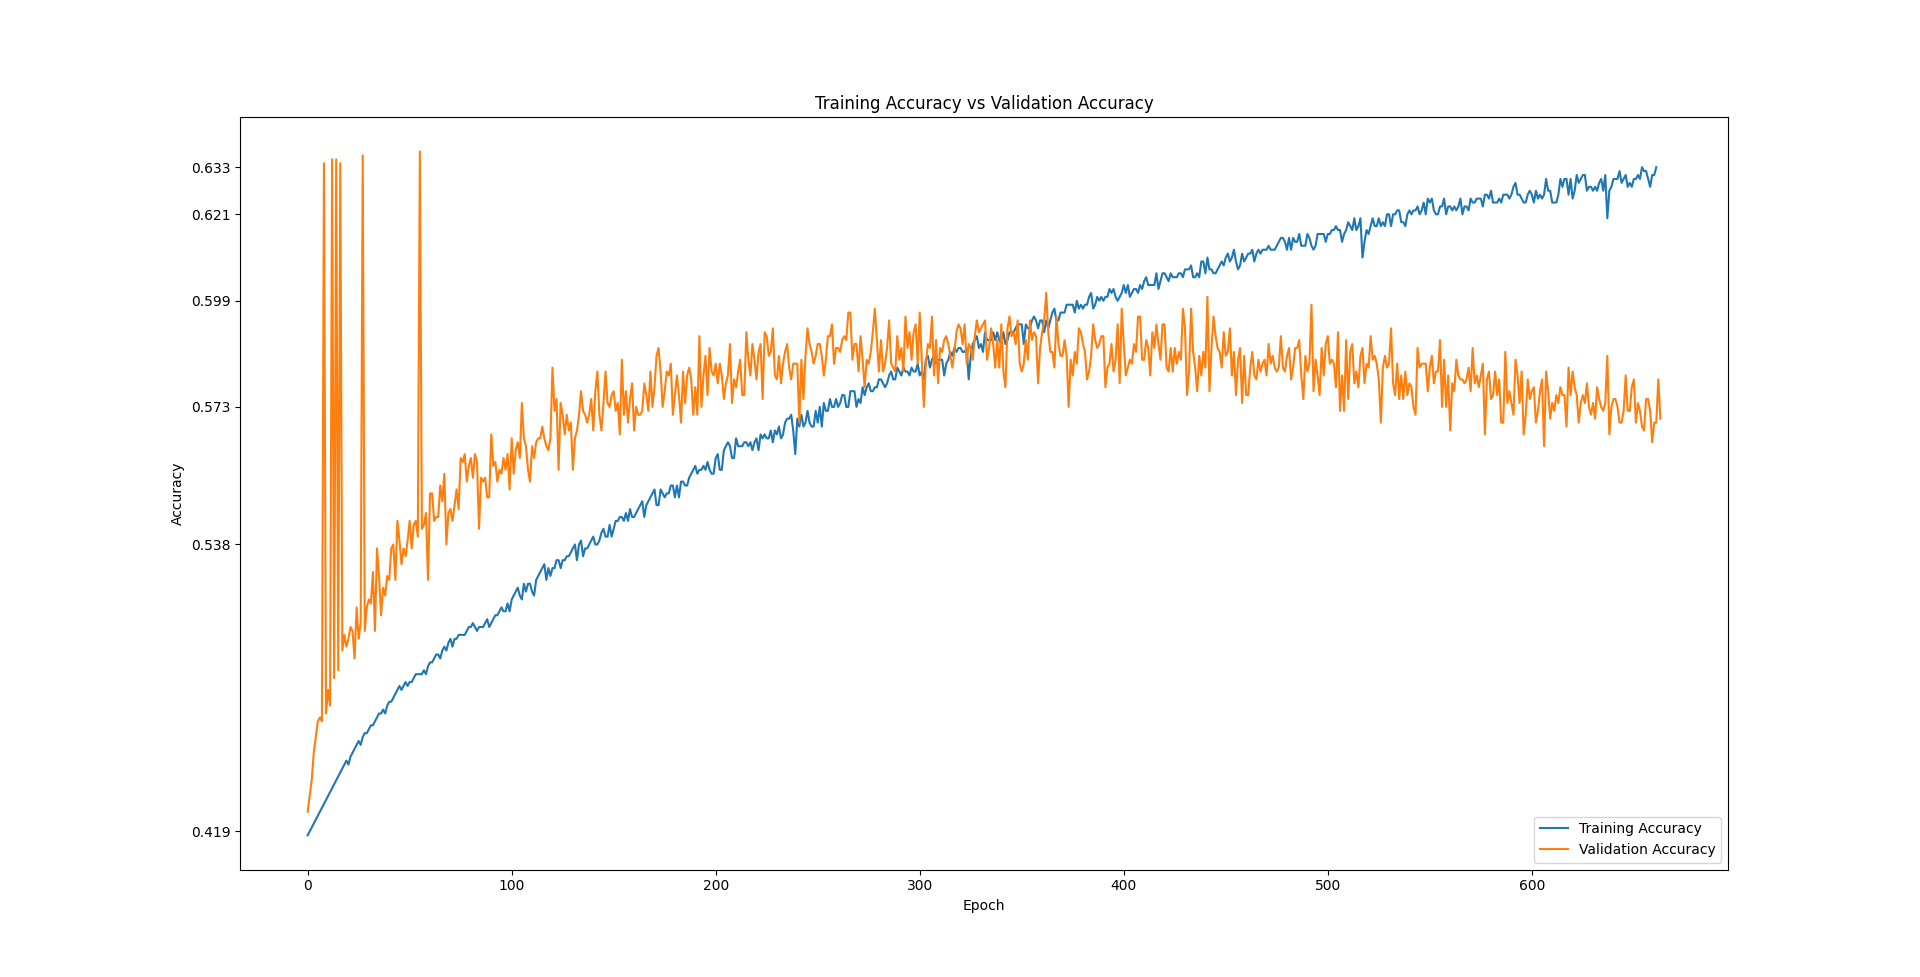
\includegraphics{train_valid_accuracy} 

}

\caption{Training Accuracy During Pre-training}\label{fig:training_accuracy}
\end{figure}

The pre-training phase took more than 21.5 days when it was stopped for
the purpose of fine-tuning, there was no early-sopping and the change in
validation accuracy was as low as 0.002. Since the pre-training phase on
the monolingual dataset was computationally expensive and had low
accuracy, it was decided to choose a cross-lingual pre-trained model.
Therefore, the fine-tuning for this model was also stopped before it was
finished.

\hypertarget{the-result-of-the-pre-trained-xlsr-model}{%
\subsection{The result of the pre-trained XLSR
model}\label{the-result-of-the-pre-trained-xlsr-model}}

\begin{figure}

{\centering 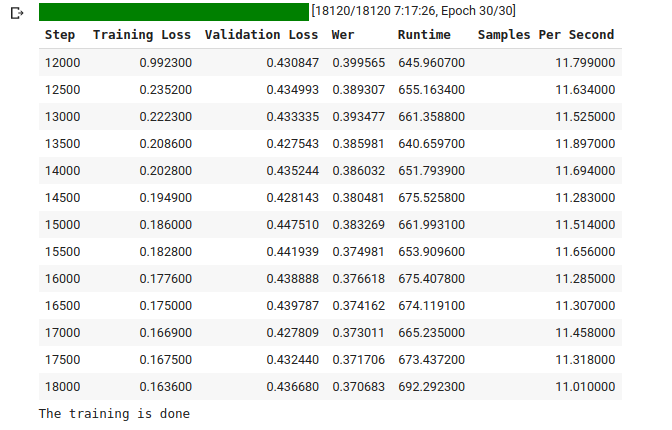
\includegraphics{training_is_done} 

}

\caption{Training Loss, Validation Loss, and WER of Training + Validation Datasets}\label{fig:wer37}
\end{figure}

Figure \ref{fig:wer37} illustrates how WER decrease as the number of
epochs and steps increases, it also shows how the training and
validation losses decrease, as well as the number of steps.

\begin{figure}

{\centering 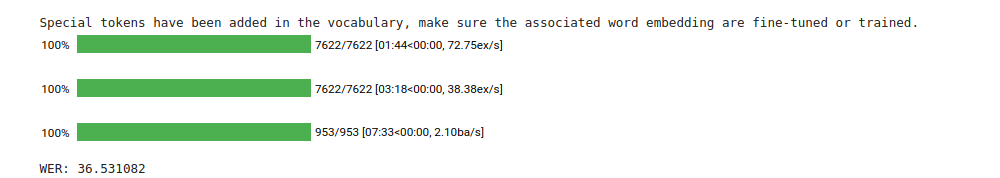
\includegraphics{WER36.53} 

}

\caption{WER Result for Test Dataset}\label{fig:WER36.53}
\end{figure}

Figure \ref{fig:WER36.53} shows the word error rate with 250 warmup
steps, \emph{3e-4} learning rate, batch size of 8, gradient accumulation
of 8 steps, and we evaluate the model every 400 steps.

\begin{figure}

{\centering 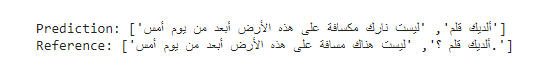
\includegraphics{sample_prediction} 

}

\caption{Sample Prediction with 0.369 WER}\label{fig:sample_prediction}
\end{figure}

Figure \ref{fig:sample_prediction} shows the predicted sentence for one
of the audio files from the test dataset. As it can be seen in figure
\ref{fig:sample_prediction} the predicted sentence and the source
sentence (Reference) are almost the same except for two words. One of
the two words is altered by \emph{Insertion} and the second word is
changed by both \emph{Deletion} and \emph{Insertion} in terms of WER
estimation.

Figure \ref{fig:wer_compared} shows different models with WER that are
compared with each other based on WER, as we can see our model placed
third with WER of 36.69 \%
\protect\hyperlink{ref-paperswithcode}{{[}61{]}}. The first model is
derived from the second model by fine-tuning the model hyperparameters.

\begin{figure}

{\centering 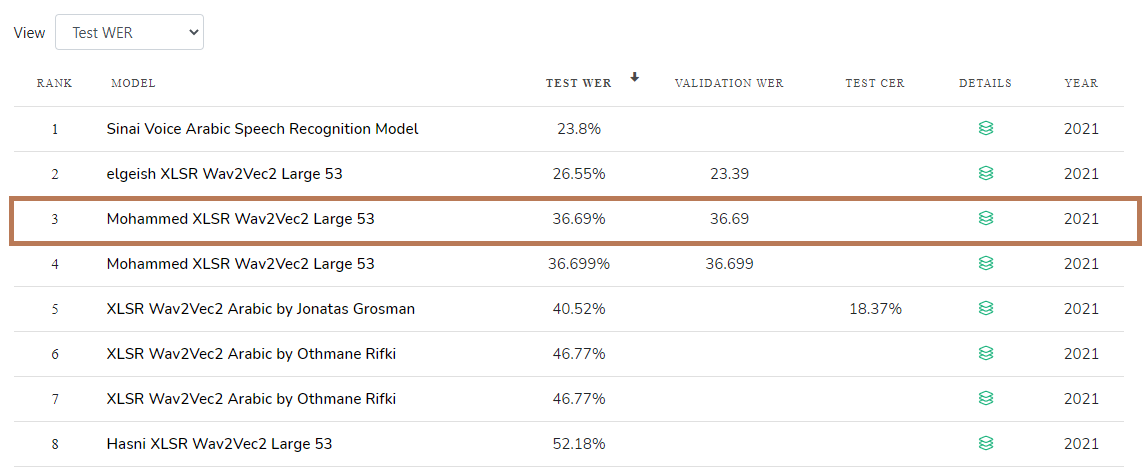
\includegraphics{wer_compared} 

}

\caption{A comparison between different fine-tuned models}\label{fig:wer_compared}
\end{figure}

\newpage

\hypertarget{discussion}{%
\section{Discussion}\label{discussion}}

Self-supervised learning provides a great way of making use of unlabeled
datasets. The data that is used for this research is unlabeled data for
the pre-training phase and labeled data for fine-tuning. SSL had been
there, before the introduction of wav2vec framework, to automatically
generate supervisory signals from unlabeled data to solve a task (a
contrastive one in our research). But it was not until wav2vec was
introduced in September 2019 by Facebook AI Research, that we have seen
a significant improvement in SSL application in speech recognition.
wav2vec is a CNN that takes raw audio as input and produces general
representations that could be used as input to an ASR. It accomplishes
that by solving a contrastive task that requires differentiating between
the true future label from negative ones. As oppose to phoneme
classification, the learned representations are applied to improve ASR
systems.

Performing a pre-training task on a single language model with a single
input language is nowhere near as accurate as pre-training ASR models on
a cross-lingual language model pre-training. This was proven by Facebook
AI Research \protect\hyperlink{ref-lample2019crosslingual}{{[}52{]}},
and was also seen clearly when we pre-trained our model on only Arabic
input, which resulted in 58\% accuracy during pre-training, and that was
a good reason for not fine-tuning the model on labeled data as the
contrastive loss is high. This could be attributed to: firstly, the huge
amount of training data for cross-lingual model one could acquire as
opposed to finding a monolingual model dataset. Secondly, as the humans'
sound-generating system is designed in the same way, it does make sense
to use other languages, with the target language that we want to
fine-tune our model on, to pre-train a model then fine-tune that model
on that target language alone.

Moreover, the process of having pre-trained models for each language for
the purpose of fine-tuning these models on languages they were
pre-trained on is time-consuming and resource-intensive. It could be
seen from our pre-training phase that more than 21 days were taken to
pre-train our model (21.5 days) without convergence. Despite the Nvidia
Tesla G80 GPU that was used for pre-training.

Fine-tuning our model on the same dataset (Mozilla Common Voice) with
different diacritics removal techniques and model parameters has
resulted in a different dictionary and a higher accuracy compared to
other models fine-tuned on the same datasets, but with different
diacritics removal techniques. There are many diacritics in the Arabic
language that need to be removed before in the preprocessing step before
doing any model training, these diacritics could be difficult to number,
and that is the reason we saw different models scoring low WER despite
them having excellent hyperparameter tuning. For instance, one of the
models uploaded on huggingface.co is reported to have had WER of 46.77
\% \protect\hyperlink{ref-Huggingface_othrif}{{[}62{]}}, however, when
checked with our diacritics removal script on the dataset the model was
tested on, the model's accuracy increased, with a WER of 45.5.

Diacritics can be confusing and using them might lead to low accuracy
during model fine-tuning because they are neither letters nor spaces,
when they were included in the fine-tuning phase they were considered by
the model as language letters in the language dictionary. This
dictionary is stored by the framework for comparing the correct
characters and assigning codes to them. Therefore, the removal of all
diacritics from the transcript files resulted in higher accuracy and low
WER.

The model initially scored 56.22 \% WER (Figure \ref{fig:WER_after_800})
before hyperparameters tuning. After removing all diacritics and tuning
hyperparameters, our model achieved a WER of 36.69 \%. It was then
reported to be compared with other models
\protect\hyperlink{ref-themodel}{{[}63{]}}. This accuracy placed our
model on the top three Arabic language models used in huggingface speech
recognition \protect\hyperlink{ref-paperswithcode}{{[}61{]}}, after a
model that scored 26.55 for WER, and another model that was tuned with
different hyper-parameters, thus, decreased the WER to 23.8 \%.

\begin{figure}

{\centering 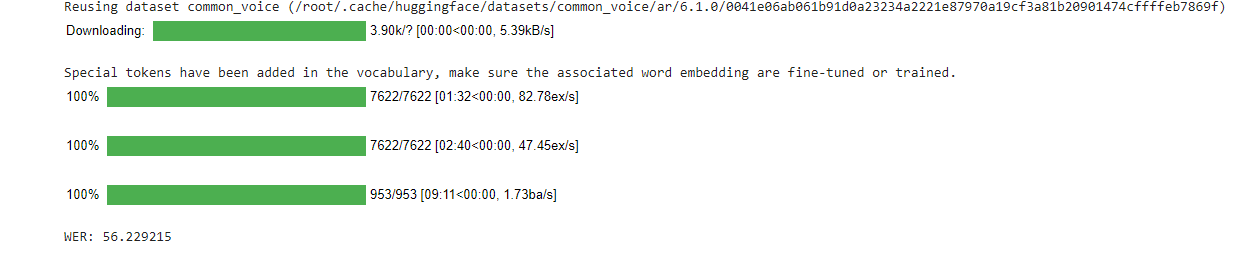
\includegraphics{WER_after_800} 

}

\caption{Initial WER before hyperparameters fine-tuning}\label{fig:WER_after_800}
\end{figure}

The model that scored the best accuracy used \emph{transliteration},
which is the process of changing a word from the alphabet of its
original language (source language) to another language (target
language). By performing transliteration on Arabic (changing all its
letters to their corresponding English letters), avoidance of diacritics
problem is for certain as we no longer have diacritics. However, having
manually removed diacritics from Arabic has also resulted in high
accuracy compared to other models.

This model could have been improved and other models could have been
developed with a different number of network layers, different vector
quantization techniques, or different language models. But due to the
limited time allocated for this thesis, it was not possible to use other
models.

\newpage

\hypertarget{conclusion}{%
\section{Conclusion}\label{conclusion}}

In this project, an Automatic Speech Recognition (ASR) system was
implemented based on a small amount of data for Arabic language.
Self-supervised learning (SSL) was the main means used for conducting
this research. A pre-training phase was, first, carried out on 42 hours
of unlabeled Arabic language dataset from \emph{Mozilla Common Voice}
for the purpose of fine-tuning this pre-trained model on labeled Arabic
data, the pre-training took more than 21 days without finishing. Due to
this, attention was instead directed to using a pre-trained model
available online. This study, secondly, took advantage of an
unsupervised cross-lingual speech representation (XLSR) that had been
pre-trained on multiple languages, including Arabic, and then this
pre-trained model was fine-tuned on Arabic language. The unsupervised
XLSR was pre-trained on 53 different languages and built on
\emph{wav2vec 2.0} which solves a contrastive task for masked latent
speech representations. This model was proven to be significantly more
efficient than the monolingual pre-training.

The Word Error Rate (WER) of the fine-tuned \emph{XLSR} with
\emph{wav2vec 2.0} on Arabic language was initially 54.00 \%. After
fine-tuning the model parameters, we obtained a WER of 36.69 \% which
placed this model third in \emph{huggingface} company's Arabic language
models. It is now being used and has been downloaded 32 times from the
official website of \emph{huggingface}
(\url{https://huggingface.co/mohammed/ar}).

The first research question is about the scarcity of transcribed data,
which is addressed by open-source projects such as \emph{Mozilla Common
Voice} that enables communities to participate in creating speech corpus
for different languages. The speech data used in this study was obtained
from \emph{Mozilla Common Voice}. Additionally, finding a huge amount of
labeled data has become no longer a concern given \emph{self-supervised
learning} (SSL). SSL, which is our second question of this research, has
proven successful when dealing with unlabeled Arabic speech data.
Cross-lingual speech representation (XLSR) was used in this research to
utilize unlabeled data from multiple languages in the pre-training phase
and then fine-tune our model on labeled Arabic language data. Using
pre-trained models for Automatic Speech Recognition, and fine-tuning
them on labeled Arabic speech data, was more efficient and time-saving
than pre-training a monolingual model. The third question takes the
model accuracy given the amount of labeled data used, and we proved that
by using as few as 42 hours of labeled data we could achieve a WER of
36.69 \%.

\newpage

\hypertarget{future-work}{%
\section{Future Work}\label{future-work}}

Data augmentation is one of the techniques that was not used in this
research and could be used to decrease WER. It is implemented by
cropping audio sequences of a predefined length when creating batches.
This method could increase the performance if all cropped audio
(sequences) have the same length. However, if the maximum length for
different audio sequences is different, then it might result in a worse
accuracy \protect\hyperlink{ref-schneider2019wav2vec}{{[}51{]}}.
Increasing the amount of unlabeled data for pre-training or labeled data
fine-tuning would also increase the model accuracy.\emph{wav2vec
Unsupervised} (\emph{wav2vec-U}) can be used to train speech recognition
models without labeled data, it leverages self-supervised speech
representations to segment unlabeled audio and learn a mapping from
these representations to phonemes via adversarial training
\protect\hyperlink{ref-baevski2021unsupervised}{{[}64{]}}.

\newpage

\hypertarget{references}{%
\section{References}\label{references}}

\setlength{\parindent}{0pt}

\hypertarget{refs}{}
\begin{CSLReferences}{0}{0}
\leavevmode\hypertarget{ref-shrawankar2013adverse}{}%
\CSLLeftMargin{{[}1{]} }
\CSLRightInline{U. Shrawankar and V. Thakare, {``Adverse conditions and
ASR techniques for robust speech user interface.''} 2013, {[}Online{]}.
Available: \url{http://arxiv.org/abs/1303.5515}.}

\leavevmode\hypertarget{ref-2020arXiv200611477B}{}%
\CSLLeftMargin{{[}2{]} }
\CSLRightInline{A. Baevski, H. Zhou, A. Mohamed, and M. Auli,
{``{wav2vec 2.0: A Framework for Self-Supervised Learning of Speech
Representations},''} \emph{arXiv e-prints}, p. arXiv:2006.11477, Jun.
2020, {[}Online{]}. Available: \url{http://arxiv.org/abs/2006.11477}.}

\leavevmode\hypertarget{ref-hannun2014deep}{}%
\CSLLeftMargin{{[}3{]} }
\CSLRightInline{A. Hannun \emph{et al.}, {``Deep speech: Scaling up
end-to-end speech recognition.''} 2014, {[}Online{]}. Available:
\url{http://arxiv.org/abs/1412.5567}.}

\leavevmode\hypertarget{ref-Mozilla}{}%
\CSLLeftMargin{{[}4{]} }
\CSLRightInline{{``Mozilla common voice.''}
\url{https://commonvoice.mozilla.org/en/about}.}

\leavevmode\hypertarget{ref-hmm}{}%
\CSLLeftMargin{{[}5{]} }
\CSLRightInline{L. R. Rabiner and B. H. Juang, {``Hidden markov models
for speech recognition --- strengths and limitations,''} in \emph{Speech
recognition and understanding}, 1992, pp. 3--29.}

\leavevmode\hypertarget{ref-1369308}{}%
\CSLLeftMargin{{[}6{]} }
\CSLRightInline{P. Pujol, S. Pol, C. Nadeu, A. Hagen, and H. Bourlard,
{``Comparison and combination of features in a hybrid HMM/MLP and a
HMM/GMM speech recognition system,''} \emph{IEEE Transactions on Speech
and Audio Processing}, vol. 13, no. 1, pp. 14--22, 2005, doi:
\href{https://doi.org/10.1109/TSA.2004.834466}{10.1109/TSA.2004.834466}.}

\leavevmode\hypertarget{ref-6681449}{}%
\CSLLeftMargin{{[}7{]} }
\CSLRightInline{L. Li \emph{et al.}, {``Hybrid deep neural
network--hidden markov model (DNN-HMM) based speech emotion
recognition,''} in \emph{2013 humaine association conference on
affective computing and intelligent interaction}, 2013, pp. 312--317,
doi: \href{https://doi.org/10.1109/ACII.2013.58}{10.1109/ACII.2013.58}.}

\leavevmode\hypertarget{ref-6854824}{}%
\CSLLeftMargin{{[}8{]} }
\CSLRightInline{S. Xue, O. Abdel-Hamid, H. Jiang, and L. Dai, {``Direct
adaptation of hybrid DNN/HMM model for fast speaker adaptation in LVCSR
based on speaker code,''} in \emph{2014 IEEE international conference on
acoustics, speech and signal processing (ICASSP)}, 2014, pp. 6339--6343,
doi:
\href{https://doi.org/10.1109/ICASSP.2014.6854824}{10.1109/ICASSP.2014.6854824}.}

\leavevmode\hypertarget{ref-Ethnologue}{}%
\CSLLeftMargin{{[}9{]} }
\CSLRightInline{G. F. S. Eberhard David M. and C. D. Fennig,
{``Ethnologue: Languages of the world. Twenty-third edition. Dallas,
texas: SIL international,''} \emph{Online version:
http://www.ethnologue.com}, 2020.}

\leavevmode\hypertarget{ref-baevski2020vqwav2vec}{}%
\CSLLeftMargin{{[}10{]} }
\CSLRightInline{A. Baevski, S. Schneider, and M. Auli, {``Vq-wav2vec:
Self-supervised learning of discrete speech representations.''} 2020,
{[}Online{]}. Available: \url{http://arxiv.org/abs/1910.05453}.}

\leavevmode\hypertarget{ref-migrationpolicy}{}%
\CSLLeftMargin{{[}11{]} }
\CSLRightInline{A. Skodo, {``Sweden: By turns welcoming and restrictive
in its immigration policy,''} \emph{Online version:
https://www.migrationpolicy.org/article/sweden-turns-welcoming-and-restrictive-its-immigration-policy\#:},
2018.}

\leavevmode\hypertarget{ref-timit}{}%
\CSLLeftMargin{{[}12{]} }
\CSLRightInline{J. Garofolo \emph{et al.}, {``TIMIT acoustic-phonetic
continuous speech corpus,''} \emph{Linguistic Data Consortium}, Nov.
1992.}

\leavevmode\hypertarget{ref-phdthesis}{}%
\CSLLeftMargin{{[}13{]} }
\CSLRightInline{O. Enshassi, {``Adaptation of acoustic and language
model for improving arabic automatic speech recognition,''} PhD thesis,
2016.}

\leavevmode\hypertarget{ref-inproceedings}{}%
\CSLLeftMargin{{[}14{]} }
\CSLRightInline{E. Chang, J.-L. Zhou, S. Di, C. Huang, and K.-F. Lee,
{``Large vocabulary mandarin speech recognition with different
approaches in modeling tones.''} Jan. 2000, pp. 983--986.}

\leavevmode\hypertarget{ref-inproceedings1}{}%
\CSLLeftMargin{{[}15{]} }
\CSLRightInline{J. Ivanecký, V. Fischer, and S. Kunzmann,
{``French--german bilingual acoustic modeling for embedded voice driven
applications,''} Aug. 2005, pp. 744--744, doi:
\href{https://doi.org/10.1007/11551874_30}{10.1007/11551874\_30}.}

\leavevmode\hypertarget{ref-859138}{}%
\CSLLeftMargin{{[}16{]} }
\CSLRightInline{W. Byrne \emph{et al.}, {``Towards language independent
acoustic modeling,''} in \emph{2000 IEEE international conference on
acoustics, speech, and signal processing. Proceedings (cat.
no.00CH37100)}, 2000, vol. 2, pp. II1029--II1032 vol.2, doi:
\href{https://doi.org/10.1109/ICASSP.2000.859138}{10.1109/ICASSP.2000.859138}.}

\leavevmode\hypertarget{ref-shrawankar2013techniques}{}%
\CSLLeftMargin{{[}17{]} }
\CSLRightInline{U. Shrawankar and V. M. Thakare, {``Techniques for
feature extraction in speech recognition system : A comparative
study.''} 2013, {[}Online{]}. Available:
\url{http://arxiv.org/abs/1305.1145}.}

\leavevmode\hypertarget{ref-8949593}{}%
\CSLLeftMargin{{[}18{]} }
\CSLRightInline{H. F. Pardede, V. Zilvan, D. Krisnandi, A. Heryana, and
R. B. S. Kusumo, {``Generalized filter-bank features for robust speech
recognition against reverberation,''} in \emph{2019 international
conference on computer, control, informatics and its applications
(IC3INA)}, 2019, pp. 19--24, doi:
\href{https://doi.org/10.1109/IC3INA48034.2019.8949593}{10.1109/IC3INA48034.2019.8949593}.}

\leavevmode\hypertarget{ref-4320436}{}%
\CSLLeftMargin{{[}19{]} }
\CSLRightInline{J. W. Cooley, P. A. W. Lewis, and P. D. Welch, {``The
fast fourier transform and its applications,''} \emph{IEEE Transactions
on Education}, vol. 12, no. 1, pp. 27--34, 1969, doi:
\href{https://doi.org/10.1109/TE.1969.4320436}{10.1109/TE.1969.4320436}.}

\leavevmode\hypertarget{ref-logft}{}%
\CSLLeftMargin{{[}20{]} }
\CSLRightInline{G. V. Haines and A. G. Jones, {``{Logarithmic Fourier
transformation},''} \emph{Geophysical Journal International}, vol. 92,
no. 1, pp. 171--178, Jan. 1988, doi:
\href{https://doi.org/10.1111/j.1365-246X.1988.tb01131.x}{10.1111/j.1365-246X.1988.tb01131.x}.}

\leavevmode\hypertarget{ref-6296527}{}%
\CSLLeftMargin{{[}21{]} }
\CSLRightInline{M. J. F. Gales, S. Watanabe, and E. Fosler-Lussier,
{``Structured discriminative models for speech recognition: An
overview,''} \emph{IEEE Signal Processing Magazine}, vol. 29, no. 6, pp.
70--81, 2012, doi:
\href{https://doi.org/10.1109/MSP.2012.2207140}{10.1109/MSP.2012.2207140}.}

\leavevmode\hypertarget{ref-4815544}{}%
\CSLLeftMargin{{[}22{]} }
\CSLRightInline{J. M. Baker \emph{et al.}, {``Developments and
directions in speech recognition and understanding, part 1 {[}DSP
education{]},''} \emph{IEEE Signal Processing Magazine}, vol. 26, no. 3,
pp. 75--80, 2009, doi:
\href{https://doi.org/10.1109/MSP.2009.932166}{10.1109/MSP.2009.932166}.}

\leavevmode\hypertarget{ref-pronun}{}%
\CSLLeftMargin{{[}23{]} }
\CSLRightInline{{``Pronunciation model.''}
\url{https://maelfabien.github.io/machinelearning/speech_reco/\#pronunciation}.}

\leavevmode\hypertarget{ref-6296526}{}%
\CSLLeftMargin{{[}24{]} }
\CSLRightInline{G. Hinton \emph{et al.}, {``Deep neural networks for
acoustic modeling in speech recognition: The shared views of four
research groups,''} \emph{IEEE Signal Processing Magazine}, vol. 29, no.
6, pp. 82--97, 2012, doi:
\href{https://doi.org/10.1109/MSP.2012.2205597}{10.1109/MSP.2012.2205597}.}

\leavevmode\hypertarget{ref-862023}{}%
\CSLLeftMargin{{[}25{]} }
\CSLRightInline{Jong-Hwan Lee, Ho-Young Jung, Te-Won Lee, and Soo-Young
Lee, {``Speech feature extraction using independent component
analysis,''} in \emph{2000 IEEE international conference on acoustics,
speech, and signal processing. Proceedings (cat. no.00CH37100)}, 2000,
vol. 3, pp. 1631--1634 vol.3, doi:
\href{https://doi.org/10.1109/ICASSP.2000.862023}{10.1109/ICASSP.2000.862023}.}

\leavevmode\hypertarget{ref-sak2015fast}{}%
\CSLLeftMargin{{[}26{]} }
\CSLRightInline{H. Sak, A. Senior, K. Rao, and F. Beaufays, {``Fast and
accurate recurrent neural network acoustic models for speech
recognition.''} 2015, {[}Online{]}. Available:
\url{http://arxiv.org/abs/1507.06947}.}

\leavevmode\hypertarget{ref-5745027}{}%
\CSLLeftMargin{{[}27{]} }
\CSLRightInline{A. V. Nefian, L. Liang, X. Pi, L. Xiaoxiang, C. Mao, and
K. Murphy, {``A coupled HMM for audio-visual speech recognition,''} in
\emph{2002 IEEE international conference on acoustics, speech, and
signal processing}, 2002, vol. 2, pp. II-2013-II-2016, doi:
\href{https://doi.org/10.1109/ICASSP.2002.5745027}{10.1109/ICASSP.2002.5745027}.}

\leavevmode\hypertarget{ref-amodei2015deep}{}%
\CSLLeftMargin{{[}28{]} }
\CSLRightInline{D. Amodei \emph{et al.}, {``Deep speech 2: End-to-end
speech recognition in english and mandarin.''} 2015, {[}Online{]}.
Available: \url{http://arxiv.org/abs/1512.02595}.}

\leavevmode\hypertarget{ref-6857341}{}%
\CSLLeftMargin{{[}29{]} }
\CSLRightInline{O. Abdel-Hamid, A. Mohamed, H. Jiang, L. Deng, G. Penn,
and D. Yu, {``Convolutional neural networks for speech recognition,''}
\emph{IEEE/ACM Transactions on Audio, Speech, and Language Processing},
vol. 22, no. 10, pp. 1533--1545, 2014, doi:
\href{https://doi.org/10.1109/TASLP.2014.2339736}{10.1109/TASLP.2014.2339736}.}

\leavevmode\hypertarget{ref-Yamashita2018}{}%
\CSLLeftMargin{{[}30{]} }
\CSLRightInline{R. Yamashita, M. Nishio, R. K. G. Do, and K. Togashi,
{``Convolutional neural networks: An overview and application in
radiology,''} \emph{Insights into Imaging}, vol. 9, no. 4, pp. 611--629,
Aug. 2018, doi:
\href{https://doi.org/10.1007/s13244-018-0639-9}{10.1007/s13244-018-0639-9}.}

\leavevmode\hypertarget{ref-kernel}{}%
\CSLLeftMargin{{[}31{]} }
\CSLRightInline{{``Kernel size and strides.''}
\url{https://insightsimaging.springeropen.com/articles/10.1007/s13244-018-0639-9}.}

\leavevmode\hypertarget{ref-lemaire2019temporal}{}%
\CSLLeftMargin{{[}32{]} }
\CSLRightInline{Q. Lemaire and A. Holzapfel, {``Temporal convolutional
networks for speech and music detection in radio broadcast,''} 2019.}

\leavevmode\hypertarget{ref-tian2017deep}{}%
\CSLLeftMargin{{[}33{]} }
\CSLRightInline{X. Tian \emph{et al.}, {``Deep LSTM for large vocabulary
continuous speech recognition.''} 2017, {[}Online{]}. Available:
\url{http://arxiv.org/abs/1703.07090}.}

\leavevmode\hypertarget{ref-graves2013speech}{}%
\CSLLeftMargin{{[}34{]} }
\CSLRightInline{A. Graves, A. Mohamed, and G. Hinton, {``Speech
recognition with deep recurrent neural networks.''} 2013, {[}Online{]}.
Available: \url{http://arxiv.org/abs/1303.5778}.}

\leavevmode\hypertarget{ref-vaswani2017attention}{}%
\CSLLeftMargin{{[}35{]} }
\CSLRightInline{A. Vaswani \emph{et al.}, {``Attention is all you
need.''} 2017, {[}Online{]}. Available:
\url{http://arxiv.org/abs/1706.03762}.}

\leavevmode\hypertarget{ref-lu2020exploring}{}%
\CSLLeftMargin{{[}36{]} }
\CSLRightInline{L. Lu, C. Liu, J. Li, and Y. Gong, {``Exploring
transformers for large-scale speech recognition.''} 2020, {[}Online{]}.
Available: \url{http://arxiv.org/abs/2005.09684}.}

\leavevmode\hypertarget{ref-towardsdatasience}{}%
\CSLLeftMargin{{[}37{]} }
\CSLRightInline{R. Horev, {``BERT explained: State of the art language
model for NLP.''} 2018, {[}Online{]}. Available:
\url{https://towardsdatascience.com/bert-explained-state-of-the-art-language-model-for-nlp-f8b21a9b6270}.}

\leavevmode\hypertarget{ref-dai2019transformerxl}{}%
\CSLLeftMargin{{[}38{]} }
\CSLRightInline{Z. Dai, Z. Yang, Y. Yang, J. Carbonell, Q. V. Le, and R.
Salakhutdinov, {``Transformer-XL: Attentive language models beyond a
fixed-length context.''} 2019, {[}Online{]}. Available:
\url{http://arxiv.org/abs/1901.02860}.}

\leavevmode\hypertarget{ref-2019arXiv190612340H}{}%
\CSLLeftMargin{{[}39{]} }
\CSLRightInline{D. Hendrycks, M. Mazeika, S. Kadavath, and D. Song,
{``{Using Self-Supervised Learning Can Improve Model Robustness and
Uncertainty},''} \emph{arXiv e-prints}, p. arXiv:1906.12340, Jun. 2019,
{[}Online{]}. Available: \url{http://arxiv.org/abs/1906.12340}.}

\leavevmode\hypertarget{ref-peters2018deep}{}%
\CSLLeftMargin{{[}40{]} }
\CSLRightInline{M. E. Peters \emph{et al.}, {``Deep contextualized word
representations.''} 2018, {[}Online{]}. Available:
\url{http://arxiv.org/abs/1802.05365}.}

\leavevmode\hypertarget{ref-radford2018improving}{}%
\CSLLeftMargin{{[}41{]} }
\CSLRightInline{A. Radford, K. Narasimhan, T. Salimans, and I.
Sutskever, {``Improving language understanding by generative
pre-training,''} 2018.}

\leavevmode\hypertarget{ref-devlin2019bert}{}%
\CSLLeftMargin{{[}42{]} }
\CSLRightInline{J. Devlin, M.-W. Chang, K. Lee, and K. Toutanova,
{``BERT: Pre-training of deep bidirectional transformers for language
understanding.''} 2019, {[}Online{]}. Available:
\url{http://arxiv.org/abs/1810.04805}.}

\leavevmode\hypertarget{ref-he2020momentum}{}%
\CSLLeftMargin{{[}43{]} }
\CSLRightInline{K. He, H. Fan, Y. Wu, S. Xie, and R. Girshick,
{``Momentum contrast for unsupervised visual representation learning.''}
2020, {[}Online{]}. Available: \url{http://arxiv.org/abs/1911.05722}.}

\leavevmode\hypertarget{ref-chen2020simple}{}%
\CSLLeftMargin{{[}44{]} }
\CSLRightInline{T. Chen, S. Kornblith, M. Norouzi, and G. Hinton, {``A
simple framework for contrastive learning of visual representations.''}
2020, {[}Online{]}. Available: \url{http://arxiv.org/abs/2002.05709}.}

\leavevmode\hypertarget{ref-jiang2019improving}{}%
\CSLLeftMargin{{[}45{]} }
\CSLRightInline{D. Jiang \emph{et al.}, {``Improving transformer-based
speech recognition using unsupervised pre-training.''} 2019,
{[}Online{]}. Available: \url{http://arxiv.org/abs/1910.09932}.}

\leavevmode\hypertarget{ref-5432202}{}%
\CSLLeftMargin{{[}46{]} }
\CSLRightInline{H. Jégou, M. Douze, and C. Schmid, {``Product
quantization for nearest neighbor search,''} \emph{IEEE Transactions on
Pattern Analysis and Machine Intelligence}, vol. 33, no. 1, pp.
117--128, 2011, doi:
\href{https://doi.org/10.1109/TPAMI.2010.57}{10.1109/TPAMI.2010.57}.}

\leavevmode\hypertarget{ref-dieleman2018challenge}{}%
\CSLLeftMargin{{[}47{]} }
\CSLRightInline{S. Dieleman, A. van den Oord, and K. Simonyan, {``The
challenge of realistic music generation: Modelling raw audio at
scale.''} 2018, {[}Online{]}. Available:
\url{http://arxiv.org/abs/1806.10474}.}

\leavevmode\hypertarget{ref-agarap2019deep}{}%
\CSLLeftMargin{{[}48{]} }
\CSLRightInline{A. F. Agarap, {``Deep learning using rectified linear
units (ReLU).''} 2019, {[}Online{]}. Available:
\url{http://arxiv.org/abs/1803.08375}.}

\leavevmode\hypertarget{ref-joshi2020transfer}{}%
\CSLLeftMargin{{[}49{]} }
\CSLRightInline{V. Joshi, R. Zhao, R. R. Mehta, K. Kumar, and J. Li,
{``Transfer learning approaches for streaming end-to-end speech
recognition system.''} 2020, {[}Online{]}. Available:
\url{http://arxiv.org/abs/2008.05086}.}

\leavevmode\hypertarget{ref-m2014choice}{}%
\CSLLeftMargin{{[}50{]} }
\CSLRightInline{L. N. M. and S. K. Kopparapu, {``Choice of mel filter
bank in computing MFCC of a resampled speech.''} 2014, {[}Online{]}.
Available: \url{http://arxiv.org/abs/1410.6903}.}

\leavevmode\hypertarget{ref-schneider2019wav2vec}{}%
\CSLLeftMargin{{[}51{]} }
\CSLRightInline{S. Schneider, A. Baevski, R. Collobert, and M. Auli,
{``wav2vec: Unsupervised pre-training for speech recognition.''} 2019,
{[}Online{]}. Available: \url{http://arxiv.org/abs/1904.05862}.}

\leavevmode\hypertarget{ref-lample2019crosslingual}{}%
\CSLLeftMargin{{[}52{]} }
\CSLRightInline{G. Lample and A. Conneau, {``Cross-lingual language
model pretraining.''} 2019, {[}Online{]}. Available:
\url{http://arxiv.org/abs/1901.07291}.}

\leavevmode\hypertarget{ref-conneau2020unsupervised}{}%
\CSLLeftMargin{{[}53{]} }
\CSLRightInline{A. Conneau, A. Baevski, R. Collobert, A. Mohamed, and M.
Auli, {``Unsupervised cross-lingual representation learning for speech
recognition.''} 2020, {[}Online{]}. Available:
\url{http://arxiv.org/abs/2006.13979}.}

\leavevmode\hypertarget{ref-inproceedingsctc}{}%
\CSLLeftMargin{{[}54{]} }
\CSLRightInline{A. Graves, S. Fernández, F. Gomez, and J. Schmidhuber,
{``Connectionist temporal classification: Labelling unsegmented sequence
data with recurrent neural 'networks,''} in \emph{ICML 2006 -
Proceedings of the 23rd International Conference on Machine Learning},
Jan. 2006, vol. 2006, pp. 369--376, doi:
\href{https://doi.org/10.1145/1143844.1143891}{10.1145/1143844.1143891}.}

\leavevmode\hypertarget{ref-ctc}{}%
\CSLLeftMargin{{[}55{]} }
\CSLRightInline{{``CTC.''} \url{https://distill.pub/2017/ctc/}.}

\leavevmode\hypertarget{ref-ERRATTAHI201832}{}%
\CSLLeftMargin{{[}56{]} }
\CSLRightInline{R. Errattahi, A. El Hannani, and H. Ouahmane,
{``Automatic speech recognition errors detection and correction: A
review,''} \emph{Procedia Computer Science}, vol. 128, pp. 32--37, 2018,
doi: \url{https://doi.org/10.1016/j.procs.2018.03.005}.}

\leavevmode\hypertarget{ref-682181}{}%
\CSLLeftMargin{{[}57{]} }
\CSLRightInline{E. S. Ristad and P. N. Yianilos, {``Learning string-edit
distance,''} \emph{IEEE Transactions on Pattern Analysis and Machine
Intelligence}, vol. 20, no. 5, pp. 522--532, 1998, doi:
\href{https://doi.org/10.1109/34.682181}{10.1109/34.682181}.}

\leavevmode\hypertarget{ref-Abdou_Moussa_2018}{}%
\CSLLeftMargin{{[}58{]} }
\CSLRightInline{S. M. Abdou and A. M. Moussa, {``Arabic speech
recognition: Challenges and state of the art,''} in \emph{Computational
linguistics, speech and image processing for arabic language}, WORLD
SCIENTIFIC, 2018, pp. 1--27.}

\leavevmode\hypertarget{ref-hssini2011design}{}%
\CSLLeftMargin{{[}59{]} }
\CSLRightInline{M. Hssini and A. Lazrek, {``Design of arabic diacritical
marks.''} 2011, {[}Online{]}. Available:
\url{http://arxiv.org/abs/1107.4734}.}

\leavevmode\hypertarget{ref-kingma2017adam}{}%
\CSLLeftMargin{{[}60{]} }
\CSLRightInline{D. P. Kingma and J. Ba, {``Adam: A method for stochastic
optimization.''} 2017, {[}Online{]}. Available:
\url{http://arxiv.org/abs/1412.6980}.}

\leavevmode\hypertarget{ref-paperswithcode}{}%
\CSLLeftMargin{{[}61{]} }
\CSLRightInline{{``Othrif model huggingface.''}
\url{https://paperswithcode.com/sota/speech-recognition-on-common-voice-arabic}.}

\leavevmode\hypertarget{ref-Huggingface_othrif}{}%
\CSLLeftMargin{{[}62{]} }
\CSLRightInline{{``Othrif model huggingface.''}
\url{https://huggingface.co/othrif/wav2vec2-large-xlsr-arabic}.}

\leavevmode\hypertarget{ref-themodel}{}%
\CSLLeftMargin{{[}63{]} }
\CSLRightInline{{``The model huggingface.''}
\url{https://huggingface.co/mohammed/ar}.}

\leavevmode\hypertarget{ref-baevski2021unsupervised}{}%
\CSLLeftMargin{{[}64{]} }
\CSLRightInline{A. Baevski, W.-N. Hsu, A. Conneau, and M. Auli,
{``Unsupervised speech recognition.''} 2021, {[}Online{]}. Available:
\url{http://arxiv.org/abs/2105.11084}.}

\end{CSLReferences}

\end{document}
